
%Question 1

\begin{enumerate}[label=\thesubsection.\arabic*, ref=\thesubsection.\theenumi]
\item The 12 musical notes are given as
$C,C^\#,D,D^\#,E,F,F^\#,G,G^\#,A,A^\#,B$.
Frequency of each note is $\sqrt[12]{2}$ times the frequency of the previous note.
If the frequency of the note $C$ is 130.8 Hz, then the ratio of frequencies of notes
$F^\#$ and $C$ is: \hfill\text{(GATE BM 2025)}

\begin{multicols}{2}
\begin{enumerate}
    \setlength{\itemsep}{0pt}
    \item[(a)] $\sqrt[6]{2}$
    \item[(b)] $\sqrt{2}$
    \item[(c)] $\sqrt[4]{2}$
    \item[(d)] $2$
\end{enumerate}
\end{multicols}
\solution

Each successive musical note has a frequency
$\sqrt[12]{2}$ times that of the previous note.

From $C$ to $F^\#$, there are 6 successive intervals:

\begin{align}
C \rightarrow C^\# \rightarrow D \rightarrow D^\#
\rightarrow E \rightarrow F \rightarrow F^\#
\end{align}

From \eqref{GP}

\begin{align}
\frac{f_{F^\#}}{f_C}
=
\left(\sqrt[12]{2}\right)^6
\end{align}

\begin{align}
=2^{6/12}
=2^{1/2}
=\sqrt{2}
\end{align}

Hence,

\begin{align}
\boxed{\frac{f_{F^\#}}{f_C}=\sqrt{2}}
\end{align}


\text{The following code verifies the solution}
\begin{lstlisting}
codes/bm1.py
\end{lstlisting}

% =========================================================
% QUESTION 2
% =========================================================



\item The following figures show three curves generated using an
iterative algorithm. The total length of the curve generated after
``Iteration $n$'' is:


\hfill\text{GATE BM 2025}

% =========================================================
% ITERATION 0
% =========================================================

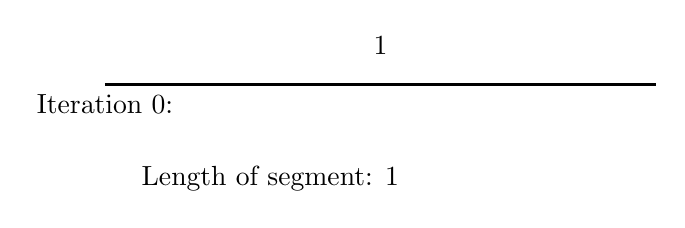
\begin{tikzpicture}[scale=1.4]

    \draw[thick] (0,0) -- (5,0);

    \node[below] at (0,0) {Iteration 0:};
    \node at (2.5,0.35) {$1$};
    \node[below] at (1.5,-0.65) {Length of segment: 1};
\end{tikzpicture}

\vspace{1.2cm}

% =========================================================
% ITERATION 1
% =========================================================
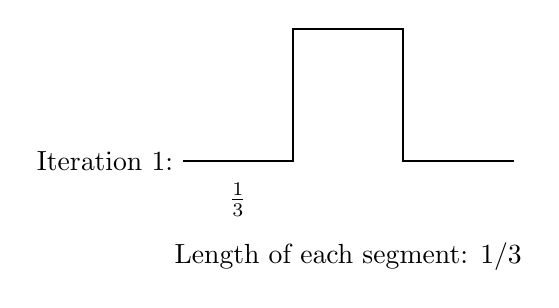
\begin{tikzpicture}[scale=1.4]

    \draw[thick]
    (0,0)
    -- (1,0)
    -- (1,1.2)
    -- (2,1.2)
    -- (2,0)
    -- (3,0);

    \node[left] at (0,0) {Iteration 1:};

    \node at (0.5,-0.35) {$\frac{1}{3}$};

    \node[below] at (1.5,-0.65) {Length of each segment: 1/3};

\end{tikzpicture}


% =========================================================
% ITERATION 2
% =========================================================
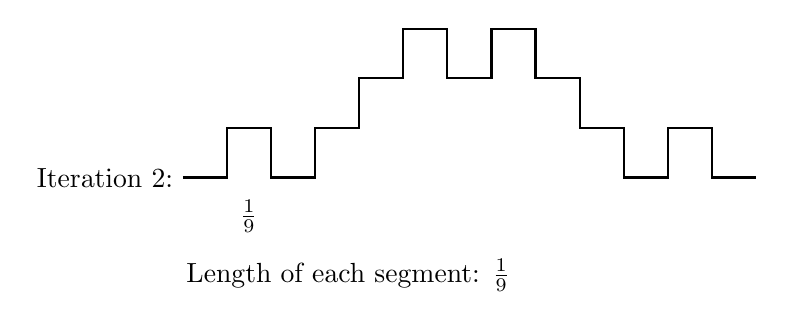
\begin{tikzpicture}[scale=1.4]

    \draw[thick]
    (0,0)
    -- (0.4,0)
    -- (0.4,0.45)
    -- (0.8,0.45)
    -- (0.8,0)
    -- (1.2,0)
    -- (1.2,0.45)
    -- (1.6,0.45)
    -- (1.6,0.9)
    -- (2.0,0.9)
    -- (2.0,1.35)
    -- (2.4,1.35)
    -- (2.4,0.9)
    -- (2.8,0.9)
    -- (2.8,1.35)
    -- (3.2,1.35)
    -- (3.2,0.9)
    -- (3.6,0.9)
    -- (3.6,0.45)
    -- (4.0,0.45)
    -- (4.0,0)
    -- (4.4,0)
    -- (4.4,0.45)
    -- (4.8,0.45)
    -- (4.8,0)
    -- (5.2,0);

    \node[left] at (0,0) {Iteration 2:};

    \node at (0.6,-0.35) {$\frac{1}{9}$};

    \node[below] at (1.5,-0.65) {Length of each segment: $\frac{1}{9}$};

\end{tikzpicture}


% =========================================================
% OPTIONS
% =========================================================
\begin{multicols}{2}
\begin{enumerate}
\setlength{\itemsep}{0pt}
    \item[(a)] $\left(\frac{5}{3}\right)^{\frac{n}{2}}$

    \item[(b)] $\left(\frac{5}{3}\right)^n$

    \item[(c)] $\left(\frac{5}{3}\right)^{2n}$

    \item[(d)] $\left(\frac{5}{3}\right)^{n(2n-1)}$
\end{enumerate}
\end{multicols}

% =========================================================
% SOLUTION
% =========================================================

\solution

At iteration $0$, the length of the curve is $1$.

\begin{align}
L_0=1
\end{align}

At iteration $1$, the curve consists of $5$ segments, each of length
$\frac{1}{3}$.

Therefore,

\begin{align}
L_1=5\left(\frac{1}{3}\right)
=\frac{5}{3}
\end{align}

At every subsequent iteration, each segment is replaced by $5$ segments,
each having $\frac{1}{3}$ of the length of the original segment.
Hence, the total length is multiplied by

\begin{align}
\frac{5}{3}
\end{align}

Therefore, after $n$ iterations,
from \eqref{iteration}


\begin{align}
L_n=\left(\frac{5}{3}\right)^n
\end{align}


% =========================================================
% QUESTION 3
% =========================================================

\item A stick of length one meter is broken at two locations at
distances of $b_1$ and $b_2$ from the origin $(0)$, as shown in the
figure. Note that $0<b_1<b_2<1$. Which one of the following is
\text{NOT} a necessary condition for forming a triangle using the
three pieces?

\text{Note:} All lengths are in meter. The figure shown is
representative.

\hfill\text{(GATE BM 2025)}

% =========================================================
% FIGURE
% =========================================================

\begin{center}

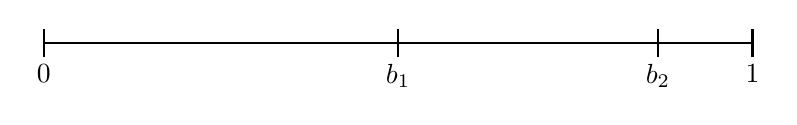
\begin{tikzpicture}[scale=1.5]

    % Main stick
    \draw[thick] (0,0) -- (6,0);

    % Tick marks
    \draw[thick] (0,-0.12) -- (0,0.12);
    \draw[thick] (3, -0.12) -- (3,0.12);
    \draw[thick] (5.2,-0.12) -- (5.2,0.12);
    \draw[thick] (6,-0.12) -- (6,0.12);

    % Labels
    \node[below=0.15cm] at (0,0) {$0$};
    \node[below=0.15cm] at (3,0) {$b_1$};
    \node[below=0.15cm] at (5.2,0) {$b_2$};
    \node[below=0.15cm] at (6,0) {$1$};

\end{tikzpicture}

\end{center}

% =========================================================
% OPTIONS
% =========================================================

\begin{multicols}{2}
\begin{enumerate}
\setlength{\itemsep}{0pt}
    \item[(a)] $b_1 < 0.5$

    \item[(b)] $b_2 > 0.5$

    \item[(c)] $b_2 < b_1 + 0.5$

    \item[(d)] $b_1+b_2 < 1$
\end{enumerate}
\end{multicols}

% =========================================================
% SOLUTION
% =========================================================

\solution

The stick of length $1$ m is broken at $b_1$ and $b_2$.

Therefore, the lengths of the three pieces are

\begin{align}
l_1=b_1,
\qquad
l_2=b_2-b_1,
\qquad
l_3=1-b_2.
\end{align}

For three lengths to form a triangle, the sum of any two sides must
be greater than the third side.

Therefore,

\begin{align}
l_1+l_2>l_3
\end{align}

\begin{align}
b_1+(b_2-b_1)>1-b_2
\end{align}

\begin{align}
b_2>1-b_2
\end{align}

\begin{align}
b_2>\frac{1}{2}.
\end{align}

Hence, option (B) is a necessary condition.

Now consider

\begin{align}
l_1+l_3>l_2.
\end{align}

Substituting the lengths,

\begin{align}
b_1+(1-b_2)>b_2-b_1.
\end{align}

Therefore,

\begin{align}
2b_1+1>2b_2
\end{align}

or

\begin{align}
b_2<b_1+\frac{1}{2}.
\end{align}

Hence, option (C) is also a necessary condition.

Finally,

\begin{align}
l_2+l_3>l_1.
\end{align}

Substituting,

\begin{align}
(b_2-b_1)+(1-b_2)>b_1.
\end{align}

Therefore,

\begin{align}
1-b_1>b_1
\end{align}

which gives

\begin{align}
b_1<\frac{1}{2}.
\end{align}

Hence, option (A) is also a necessary condition.

However, the condition

\begin{align}
b_1+b_2<1
\end{align}

is not required for the three pieces to form a triangle.

Therefore, the condition which is \textbf{NOT} necessary is (D)

\text The following code gives whether the triangle is feasible or not by taking $b_1$,$b_2$
\begin{lstlisting}
Codes/bm3.py
\end{lstlisting}


% =========================================================
% QUESTION 4
% =========================================================



\item Which one of the following represents the frequency
response of a notch filter?


\hfill \text{(GATE BM 2025)}

% =========================================================
% OPTIONS WITH GRAPHS
% =========================================================
\begin{multicols}{2}
\begin{enumerate}
\setlength{\itemsep}{0pt}
% ---------------------------------------------------------
% OPTION A
% ---------------------------------------------------------

\item[(a)]

\begin{center}
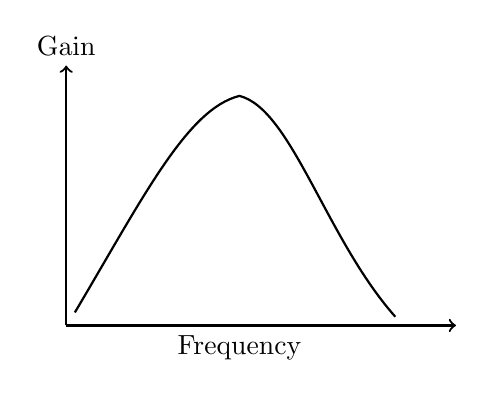
\begin{tikzpicture}[scale=1.1]

    % Axes
    \draw[->, thick] (0,0) -- (0,3);
    \draw[->, thick] (0,0) -- (4.5,0);

    % Labels
    \node[above] at (0,3) {Gain};
    \node[below] at (2,0) {Frequency};

    % Band-pass response
    \draw[thick]
        (0.1,0.15)
        .. controls (0.9,1.5) and (1.4,2.5) ..
        (2.0,2.65)
        .. controls (2.6,2.5) and (3.0,1.0) ..
        (3.8,0.1);

\end{tikzpicture}
\end{center}

% ---------------------------------------------------------
% OPTION B
% ---------------------------------------------------------

\item[(b)]

\begin{center}
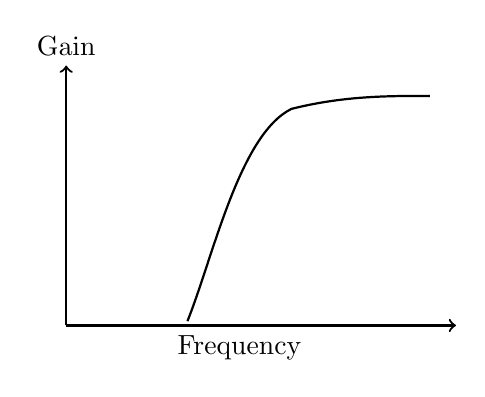
\begin{tikzpicture}[scale=1.1]

    % Axes
    \draw[->, thick] (0,0) -- (0,3);
    \draw[->, thick] (0,0) -- (4.5,0);

    % Labels
    \node[above] at (0,3) {Gain};
    \node[below] at (2,0) {Frequency};

    % High-pass response
    \draw[thick]
        (1.4,0.05)
        .. controls (1.7,0.8) and (2.0,2.2) ..
        (2.6,2.5)
        .. controls (3.2,2.65) and (3.7,2.65) ..
        (4.2,2.65);

\end{tikzpicture}
\end{center}

% ---------------------------------------------------------
% OPTION C
% ---------------------------------------------------------

\item[(c)]

\begin{center}
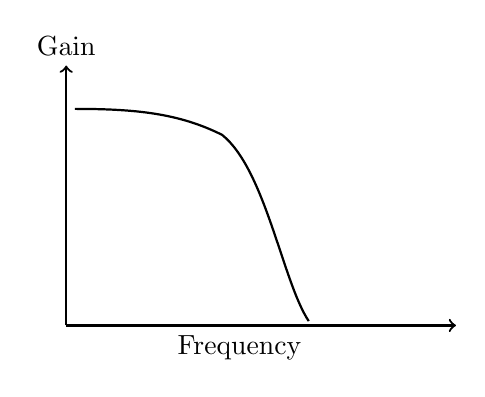
\begin{tikzpicture}[scale=1.1]

    % Axes
    \draw[->, thick] (0,0) -- (0,3);
    \draw[->, thick] (0,0) -- (4.5,0);

    % Labels
    \node[above] at (0,3) {Gain};
    \node[below] at (2,0) {Frequency};

    % Low-pass response
    \draw[thick]
        (0.1,2.5)
        .. controls (0.8,2.5) and (1.3,2.45) ..
        (1.8,2.2)
        .. controls (2.3,1.8) and (2.5,0.5) ..
        (2.8,0.05);

\end{tikzpicture}
\end{center}

% ---------------------------------------------------------
% OPTION D
% ---------------------------------------------------------

\item[(d)]

\begin{center}
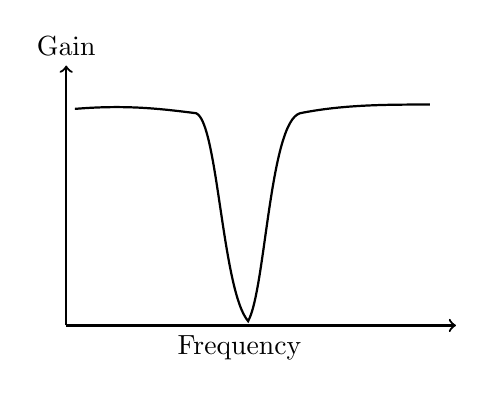
\begin{tikzpicture}[scale=1.1]

    % Axes
    \draw[->, thick] (0,0) -- (0,3);
    \draw[->, thick] (0,0) -- (4.5,0);

    % Labels
    \node[above] at (0,3) {Gain};
    \node[below] at (2,0) {Frequency};

    % Notch response
    \draw[thick]
        (0.1,2.5)
        .. controls (0.7,2.55) and (1.1,2.5) ..
        (1.5,2.45)
        .. controls (1.75,2.35) and (1.8,0.4) ..
        (2.1,0.05)
        .. controls (2.3,0.4) and (2.35,2.35) ..
        (2.7,2.45)
        .. controls (3.2,2.55) and (3.7,2.55) ..
        (4.2,2.55);

\end{tikzpicture}
\end{center}

\end{enumerate}
\end{multicols}

% =========================================================
% SOLUTION
% =========================================================

\solution

A notch filter is a band-stop filter that rejects or strongly
attenuates a narrow range of frequencies while allowing frequencies
outside that range to pass.

Therefore, its frequency response has high gain at low and high
frequencies, with a sharp reduction in gain at a particular frequency.

The response has a deep attenuation around rejected frequency.

From \eqref{freq}


Among the given frequency responses, only option (D) shows a sharp
reduction in gain at a particular frequency while allowing frequencies
on either side to pass.

% =========================================================
% QUESTION 5
% =========================================================


\item For any continuous and differentiable function $f(x)$ with
first derivative $f'(x) \neq 0$ for all values of $x$, which one of the
following is ALWAYS TRUE for $a \neq b$?

Here, $a$ and $b$ are finite and real.


\hfill \text{(GATE BM 2025)}
\begin{multicols}{2}
\begin{enumerate}
\setlength{\itemsep}{0pt}
\item[(a)] $f(a) > f(b)$


\item[(b)] $f(a) = f(b)$


\item[(c)] $f(a) \neq f(b)$

\item[(d)] $f(a) < f(b)$

\end{enumerate}
\end{multicols}


% =========================================================
% SOLUTION
% =========================================================


\solution

\noindent We are given that $f(x)$ is continuous and differentiable, and

\begin{align}
f'(x) \neq 0 \qquad \text{for all } x.
\end{align}

Suppose, for contradiction, that

\begin{align}
f(a) = f(b).
\end{align}

\noindent Since $f(x)$ is continuous on $[a,b]$ and differentiable on $(a,b)$,
\noindent Rolle's theorem can be applied.

From \eqref{rolle's}

But this contradicts the given condition

\begin{align}
f'(x)\neq0 \qquad \text{for all }x.
\end{align}

\noindent Therefore, our assumption that $f(a)=f(b)$ is false. Hence,$f(a)\neq f(b)$

% =========================================================
% QUESTION 6
% =========================================================

\item The closed loop system shown below
\underline{\hspace{2cm}}.

\begin{center}

\begin{tikzpicture}[
    >=stealth,
    block/.style={
        draw,
        rectangle,
        minimum width=4cm,
        minimum height=1.5cm
    },
    sum/.style={
        draw,
        circle,
        minimum size=0.9cm
    }
]

% Summing junction
\node[sum] (sum) {};

% Plus and minus signs
\node at ($(sum.center)+(-0.2,0.0)$) [font=\tiny] {$ +$};
\node at ($ (sum.center)+(0.2,0.0)$)[font=\tiny] {$- $};

% Input arrow
\draw[->] ($(sum.west)+(-1.2,0)$) -- (sum.west);

% Transfer function block
\node[block, right=0.8cm of sum] (G)
{
    $G(s)=\dfrac{25}{s(s+5)}$
};

% Forward path
\draw[->] (sum.east) -- (G.west);

% Output
\draw[->] (G.east) -- ++(1.2,0)
    node[right] {};

% Feedback line
\draw (G.east) -- ++(0.5,0)
    |- ($(sum.south)+(0,-1.3)$)
    -- (sum.south);

\end{tikzpicture}

\end{center}

\hfill \text{(GATE BM 2025)}
\begin{multicols}{2}
\begin{enumerate}
\setlength{\itemsep}{0pt}
\item[(a)] is overdamped


\item[(b)] is underdamped


\item[(c)] is critically damped


\item[(d)] has sustained oscillations

\end{enumerate}
\end{multicols}


% =========================================================
% SOLUTION TO QUESTION 6
% =========================================================

\solution

The forward transfer function is:
\begin{align}
G(s) = \frac{25}{s(s+5)}
\end{align}

From \eqref{neg}

Substitute $G(s)$:
\begin{align}
\frac{C(s)}{R(s)} &= \frac{\frac{25}{s(s+5)}}{1 + \frac{25}{s(s+5)}} \\
&= \frac{25}{s^2 + 5s + 25}
\end{align}

The characteristic equation in the Laplace domain is:
\begin{align}
s^2 + 5s + 25 = 0
\end{align}

Comparing this with the standard second-order system equation $s^2 + 2\zeta\omega_n s + \omega_n^2 = 0$:
\begin{align}
\omega_n^2 = 25 \implies \omega_n = 5
\end{align}
\begin{align}
2\zeta\omega_n = 5 \implies 2\zeta(5)= 5 \implies \zeta = 0.5
\end{align}

Since $0 < \zeta < 1$, From \eqref{compare} the system is underdamped.

To find the impulse response in the time domain, we compute the Inverse Laplace Transform of $C(s)$ (for $R(s) = 1$):
\begin{align}
C(s) = \frac{25}{s^2 + 5s + 25}
\end{align}

Completing the square in the denominator:
\begin{align}
s^2 + 5s + 25 &= \left(s + \frac{5}{2}\right)^2 + \frac{75}{4} \\
&= (s + 2.5)^2 + \left(\frac{5\sqrt{3}}{2}\right)^2
\end{align}

Rewriting $C(s)$:
\begin{align}
C(s) &= \frac{25}{\left(s + \frac{5}{2}\right)^2 + \left(\frac{5\sqrt{3}}{2}\right)^2}\\ &= \frac{25}{\frac{5\sqrt{3}}{2}} \cdot \frac{\frac{5\sqrt{3}}{2}}{\left(s + \frac{5}{2}\right)^2 + \left(\frac{5\sqrt{3}}{2}\right)^2}\\
&= \frac{10}{\sqrt{3}} \cdot \frac{\frac{5\sqrt{3}}{2}}{\left(s + \frac{5}{2}\right)^2 + \left(\frac{5\sqrt{3}}{2}\right)^2}
\end{align}

From \eqref{inverse}
Taking the Inverse Laplace Transform $\mathcal{L}^{-1}\{C(s)\}$:
\begin{align}
c(t) = \frac{10}{\sqrt{3}} e^{-\frac{5}{2}t} \sin\left(\frac{5\sqrt{3}}{2}t\right) \quad \text{for } t \ge 0
\end{align}

The presence of the decaying exponential $e^{-\frac{5}{2}t}$ multiplied by the sine term confirms an underdamped oscillatory response.


\begin{figure}[H]
    \centering
    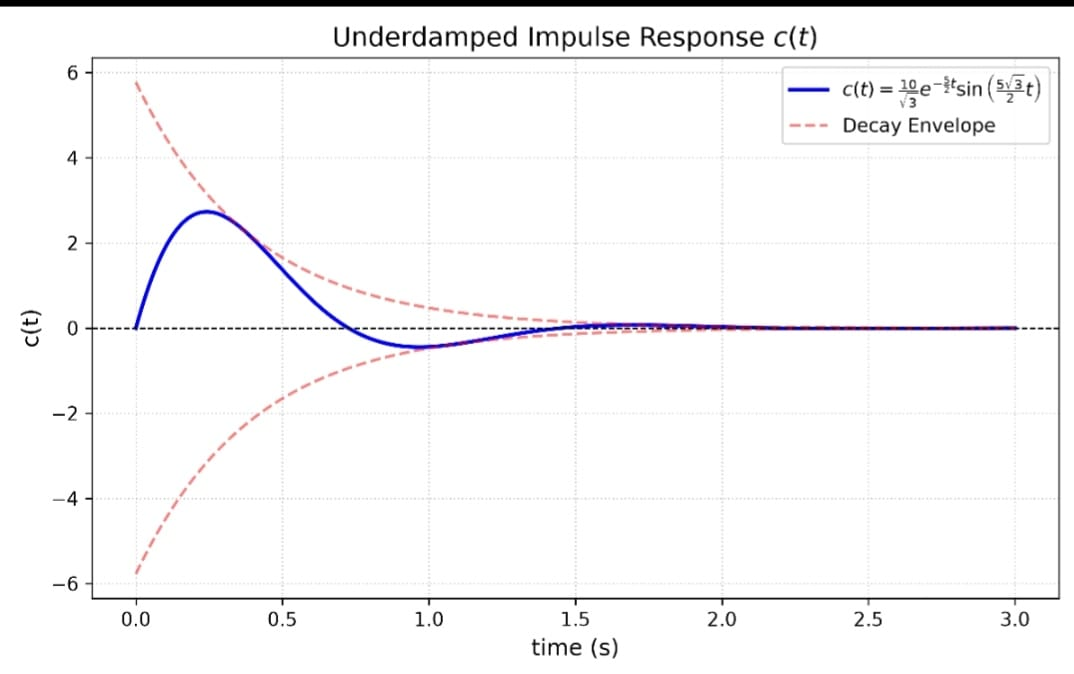
\includegraphics[width=0.75\textwidth]{figs/bm6.png}
    \caption{c(t) vs time}
    \label{c(t) vs time}
\end{figure}
\text{The following code gives the above graph}
\begin{lstlisting}
Codes/bm6.py
\end{lstlisting}

% =========================================================
% QUESTION 7
% =========================================================



\item The eigenvalues of the matrix
\begin{align}
\begin{pmatrix}
\cos\theta & -\sin\theta\\
\sin\theta & \cos\theta
\end{pmatrix}
\end{align}
are \underline{\hspace{2cm}}.


\hfill \text{(GATE BM 2025)}
\begin{multicols}{2}
\begin{enumerate}
\setlength{\itemsep}{0pt}
\item[(a)] $\cos\theta$ and $\sin\theta$

\item[(b)] $e^{i\theta}$ and $e^{-i\theta}$, where $i=\sqrt{-1}$

\item[(c)] $\cos\theta$ and $-\sin\theta$

\item[(d)] $\cos 2\theta$ and $\sin 2\theta$

\end{enumerate}
\end{multicols}

% =========================================================
% SOLUTION TO QUESTION 7
% =========================================================

\solution

Let the given matrix be

\begin{align}
\vec{A}=\myvec{
\cos\theta & -\sin\theta\\
\sin\theta & \cos\theta
}
\end{align}
\text From \eqref{eigen}


the eigenvalues are

\begin{align}
\boxed{\lambda_1=e^{i\theta},\qquad
\lambda_2=e^{-i\theta}}.
\end{align}


\text{The following code verifies the solution}
\begin{lstlisting}
Codes/bm7.py
\end{lstlisting}

% ============================================================
% QUESTION 8
% ============================================================

\item If
$
f(x)=x-\frac{1}{x},
$
the value of
$
\lim_{\Delta x\to 0}
\frac{f(1+\Delta x)-f(1)}{\Delta x}
$
is \underline{\hspace{2cm}}.
\hfill \text{(GATE BM 2025)}
\begin{multicols}{2}
\begin{enumerate}
\setlength{\itemsep}{0pt}
    \item[(a)] $0$
    
    \item[(b)] $\dfrac{1}{2}$
    
    \item[(c)] $1$
    
    \item[(d)] $2$
\end{enumerate}
\end{multicols}

%==============================================
%==============================================

\solution

The given limit is the definition of the derivative of $f(x)$ at
$x=1$:

From \eqref{derivative}
\begin{align}
f'(1)
=
\lim_{\Delta x\to 0}
\frac{f(1+\Delta x)-f(1)}{\Delta x}.
\end{align}

Given
\begin{align}
f(x)=x-\frac{1}{x},
\end{align}

differentiate with respect to $x$:

\begin{align}
f'(x)=1+\frac{1}{x^2}.
\end{align}

Therefore,

\begin{align}
f'(1)
=
1+\frac{1}{1^2}
=
2.
\end{align}


\begin{figure}[H]
    \centering
    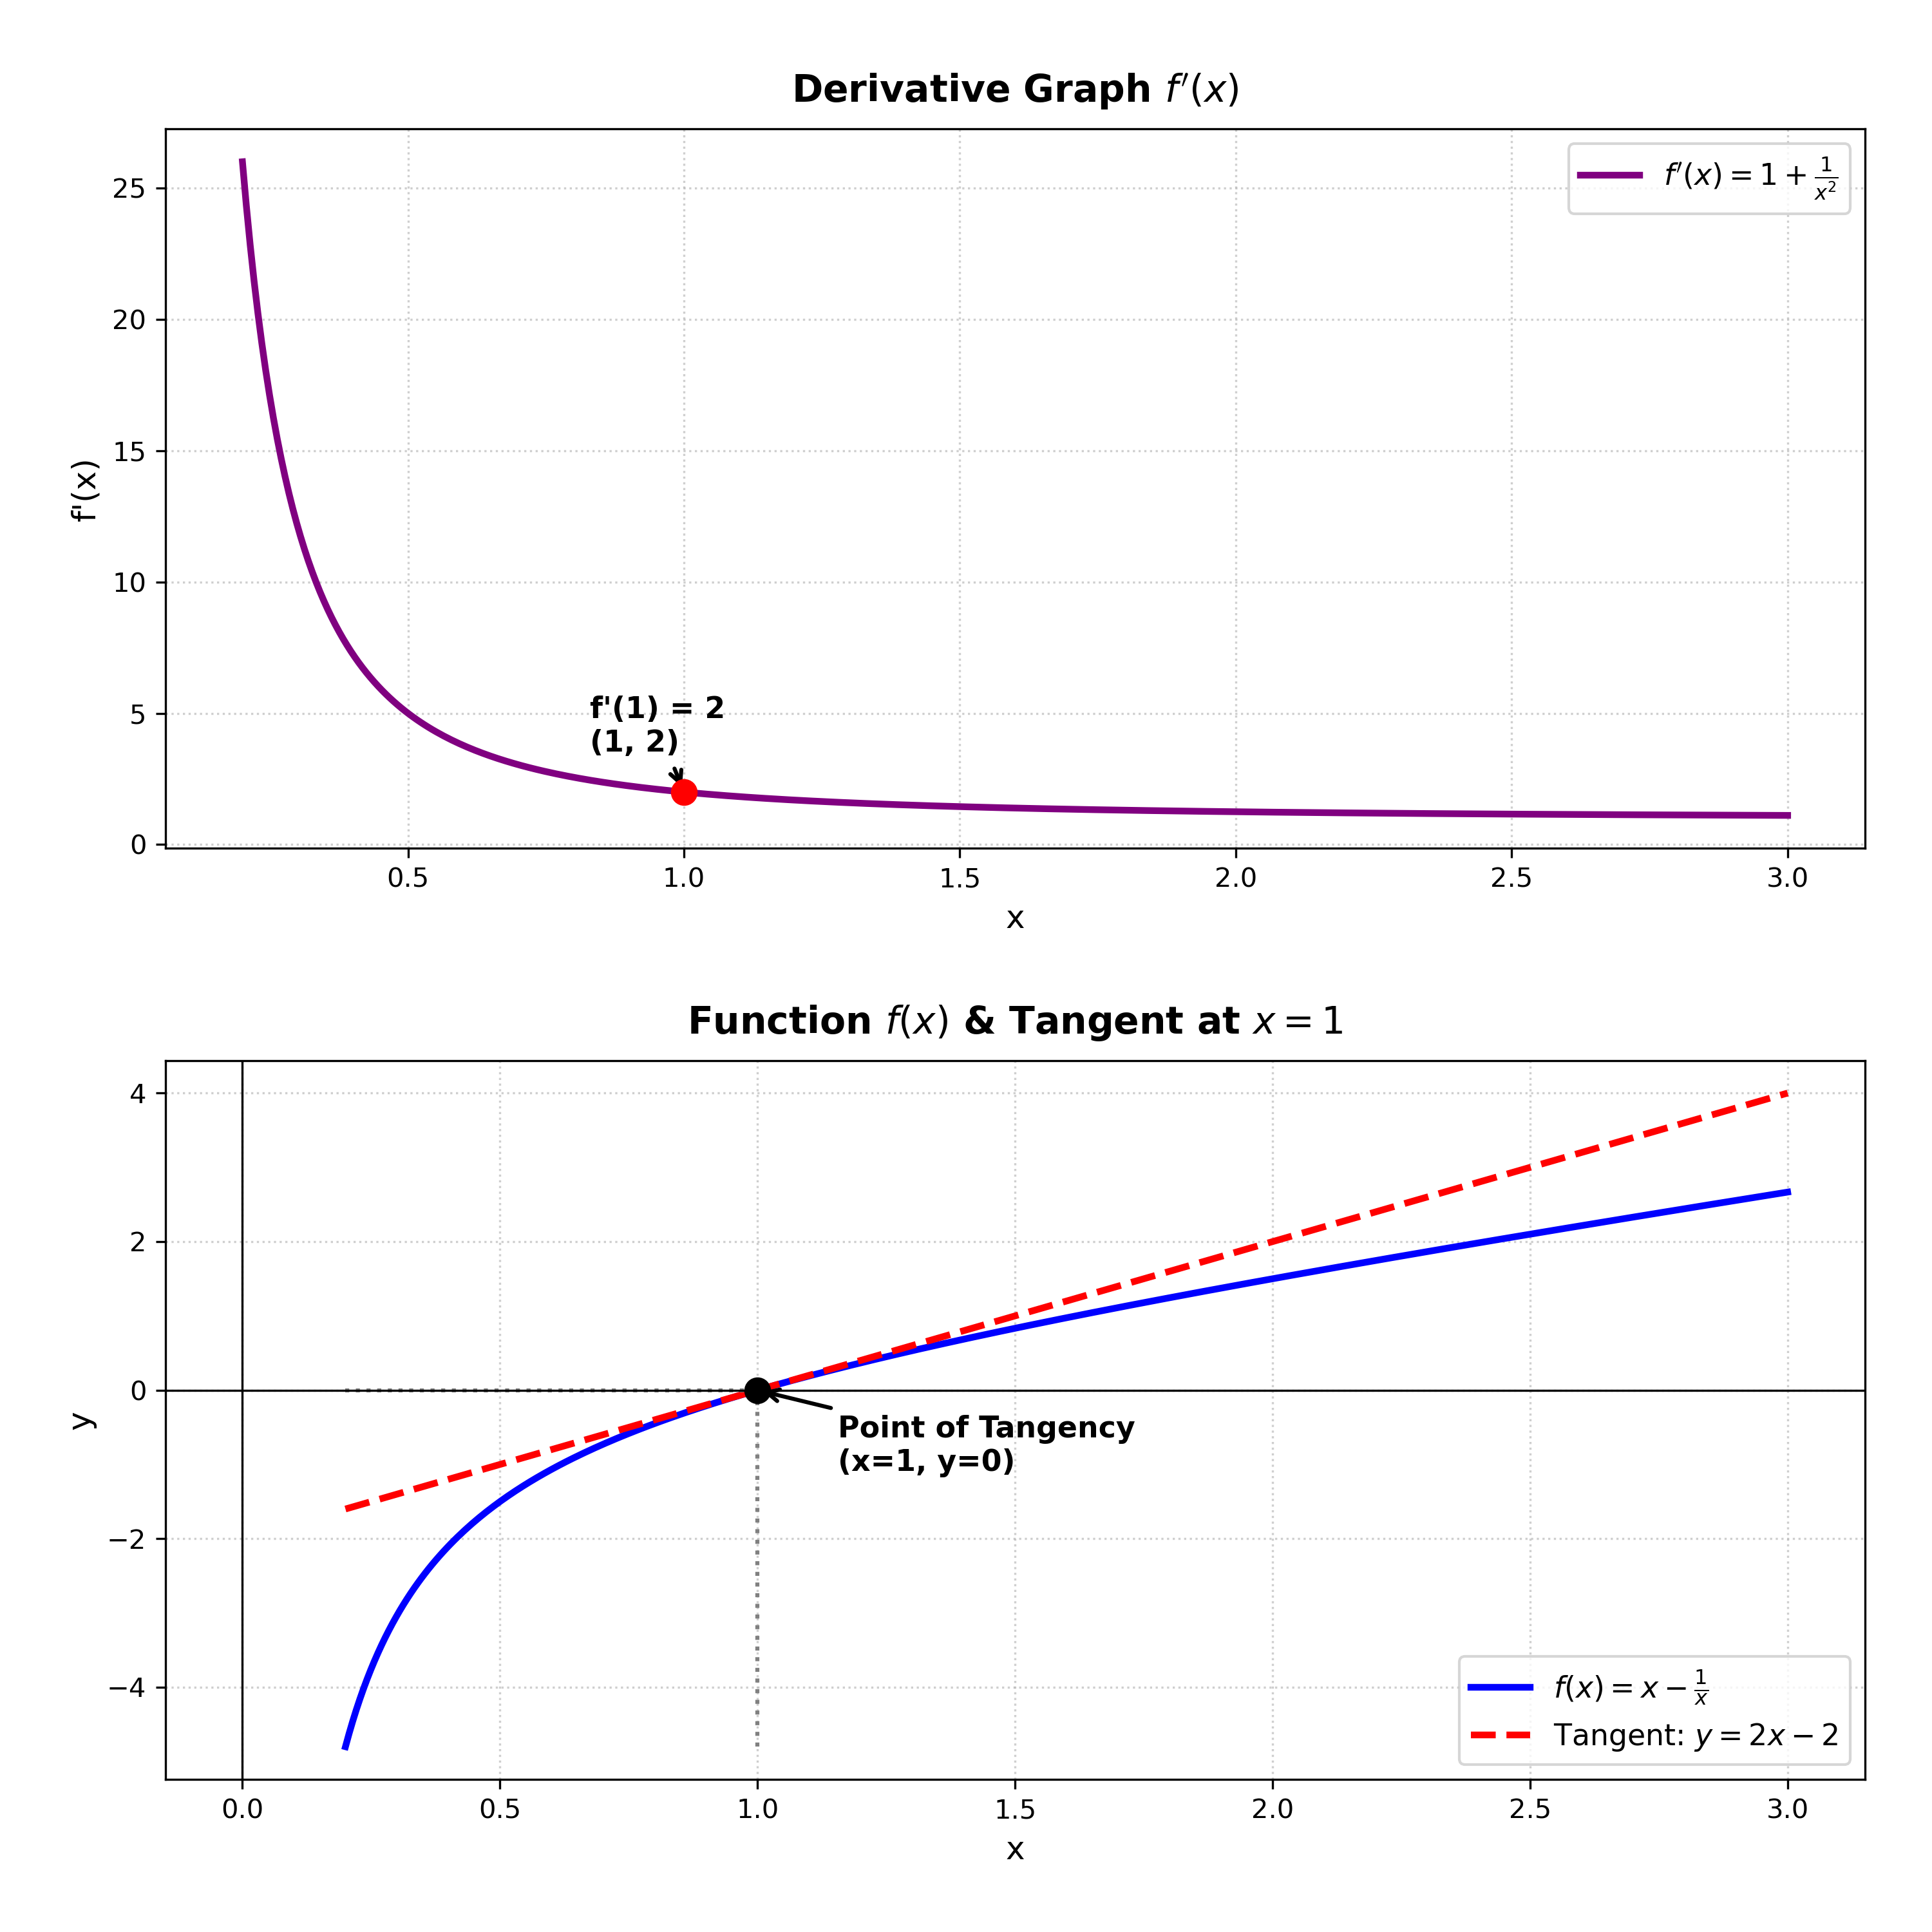
\includegraphics[width=1\textwidth]{figs/bm8a.png}
    \caption{Derivative vs x; function vs x with tangent}
    \label{Derivative vs x; function vs x with tangent}
\end{figure}

\text{The following code results the graph}
\begin{lstlisting}
Codes/bm8.py
\end{lstlisting}

% =========================================================
% QUESTION 9
% =========================================================

\item The elements of the dataset $\{-5, 1, a, 5, b\}$ are in ascending order. If both mean and median of the dataset are equal to $3$, what is the value of $b$?
\hfill \text{(GATE BM 2025)}

% =========================================================
% OPTIONS
% =========================================================
\begin{multicols}{2}
\begin{enumerate}
\setlength{\itemsep}{0pt}
    \item[(a)] $7$

    \item[(b)] $11$

    \item[(c)] $9$

    \item[(d)] $12$
\end{enumerate}
\end{multicols}

% =========================================================
% SOLUTION
% =========================================================

\solution

The dataset consists of $5$ elements arranged in ascending order:

\begin{align}
-5 \le 1 \le a \le 5 \le b
\end{align}
From \eqref{median}
Since the dataset has an odd number of elements ($n=5$), the median is the middle (3rd) element:

\begin{align}
\text{Median} = a = 3
\end{align}

The mean of the dataset is given as $3$:
From \eqref{mean}
\begin{align}
\text{Mean} = \frac{-5 + 1 + a + 5 + b}{5} = 3
\end{align}

Substituting $a = 3$ into equation (9.3):

\begin{align}
\frac{-5 + 1 + 3 + 5 + b}{5} = 3
\end{align}

\begin{align}
\frac{4 + b}{5} = 3
\end{align}

\begin{align}
4 + b = 15
\end{align}

\begin{align}
b = 11
\end{align}


\text{The following code verifies the solution}
\begin{lstlisting}
Codes/bm9.py
\end{lstlisting}


% =========================================================
% QUESTION 10
% =========================================================

\item A time domain signal is given by
\begin{align}
x(t) = 20\sin(100\pi t) + 36\sin(150\pi t) - 2\sin(300\pi t),
\end{align}
where time $t$ is in seconds. Among the following options, what is the frequency (in $\text{Hz}$) at which $x(t)$ should be sampled for accurate signal reconstruction?
\hfill \text{(GATE BM 2025)}

% =========================================================
% OPTIONS
% =========================================================

\begin{multicols}{2}
\begin{enumerate}
\setlength{\itemsep}{0pt}
    \item[(a)] $500$

    \item[(b)] $150$

    \item[(c)] $200$

    \item[(d)] $250$
\end{enumerate}
\end{multicols}

% =========================================================
% SOLUTION
% =========================================================

\solution
From \eqref{sampling}

\begin{figure}[H]
    \centering
    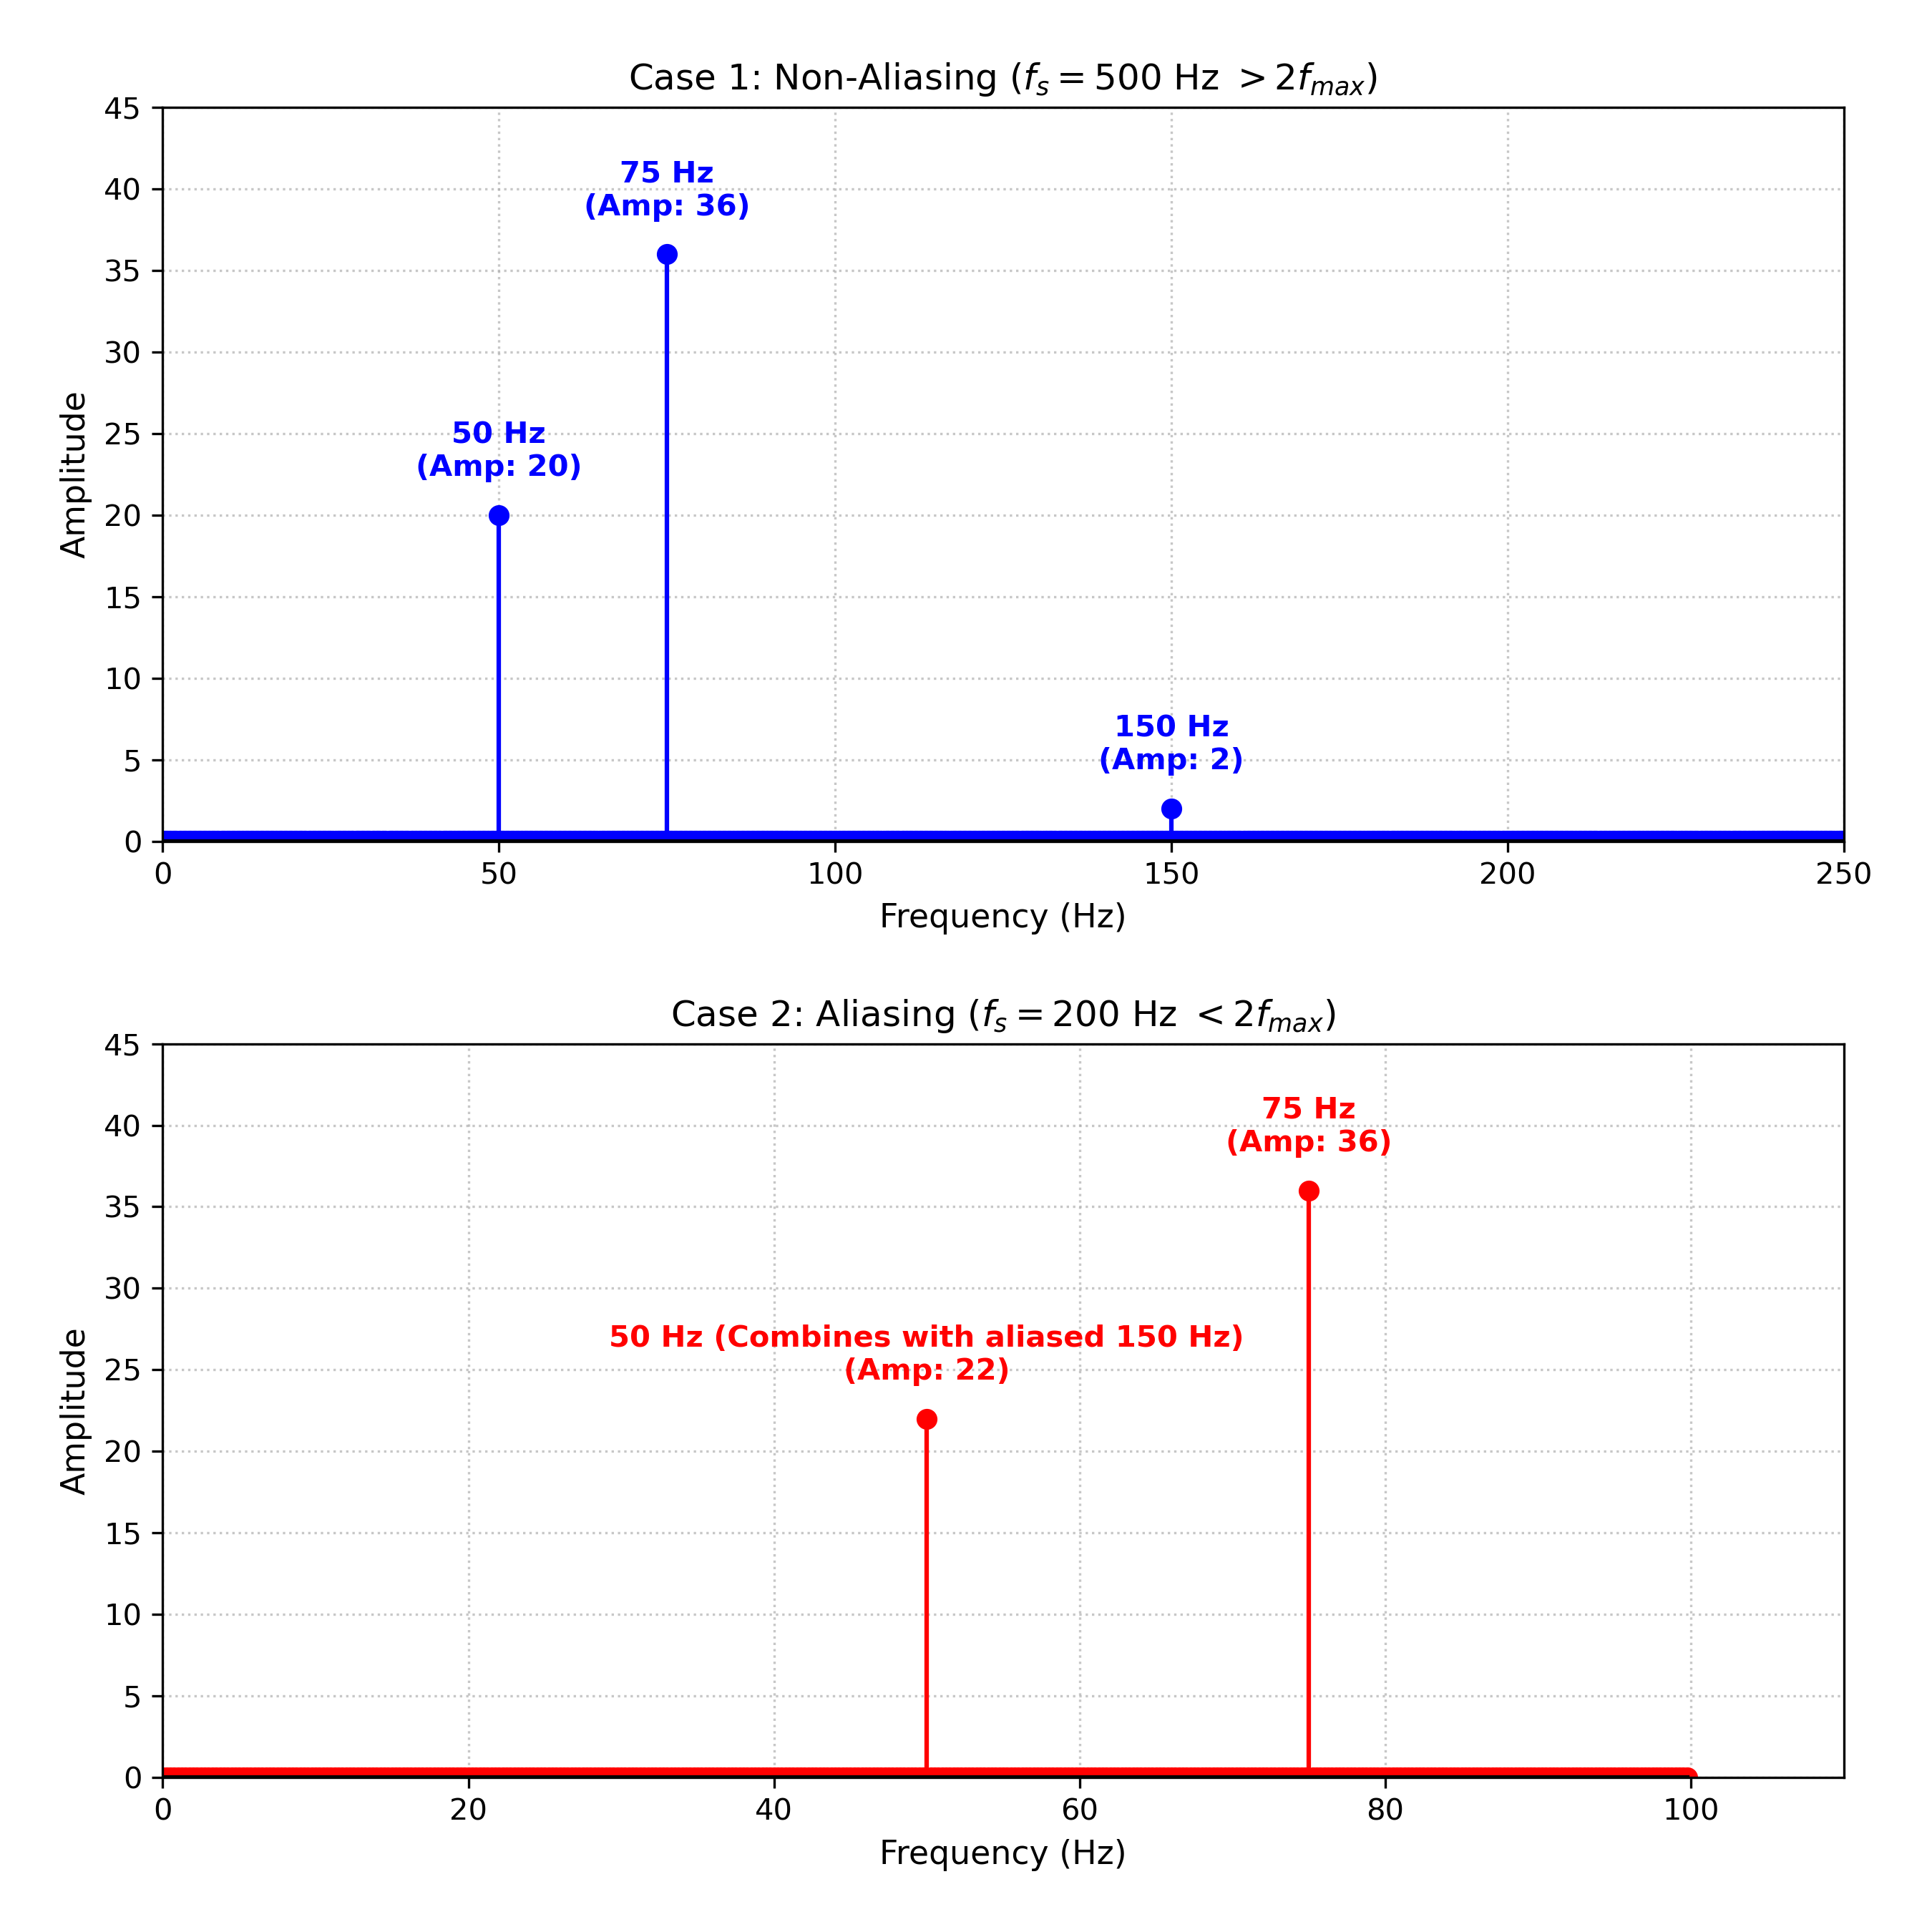
\includegraphics[width=1\columnwidth]{figs/bm10a.png}
    \caption{Aliasing and Non-Aliasing}
    \label{Aliasing and Non-Aliasing}
\end{figure}
\text{The following code results the graph}
\begin{lstlisting}
Codes/bm10a.py
\end{lstlisting}


The signal consists of three sinusoidal components with angular frequencies $\omega_1$, $\omega_2$, and $\omega_3$:

\begin{align}
\omega_1 = 100\pi \implies f_1 = \frac{100\pi}{2\pi} = 50\text{ Hz}
\end{align}

\begin{align}
\omega_2 = 150\pi \implies f_2 = \frac{150\pi}{2\pi} = 75\text{ Hz}
\end{align}

\begin{align}
\omega_3 = 300\pi \implies f_3 = \frac{300\pi}{2\pi} = 150\text{ Hz}
\end{align}

The maximum frequency component present in the signal is:

\begin{align}
f_{\max} = 150\text{ Hz}
\end{align}

According to the Nyquist theorem, the minimum required sampling rate (Nyquist rate) is:

\begin{align}
f_s \ge 2 \times 150\text{ Hz} = 300\text{ Hz}
\end{align}

Among the given options, the only frequency greater than or equal to $300\text{ Hz}$ that guarantees accurate signal reconstruction is $500\text{ Hz}$.


\begin{figure}[H]
    \centering
    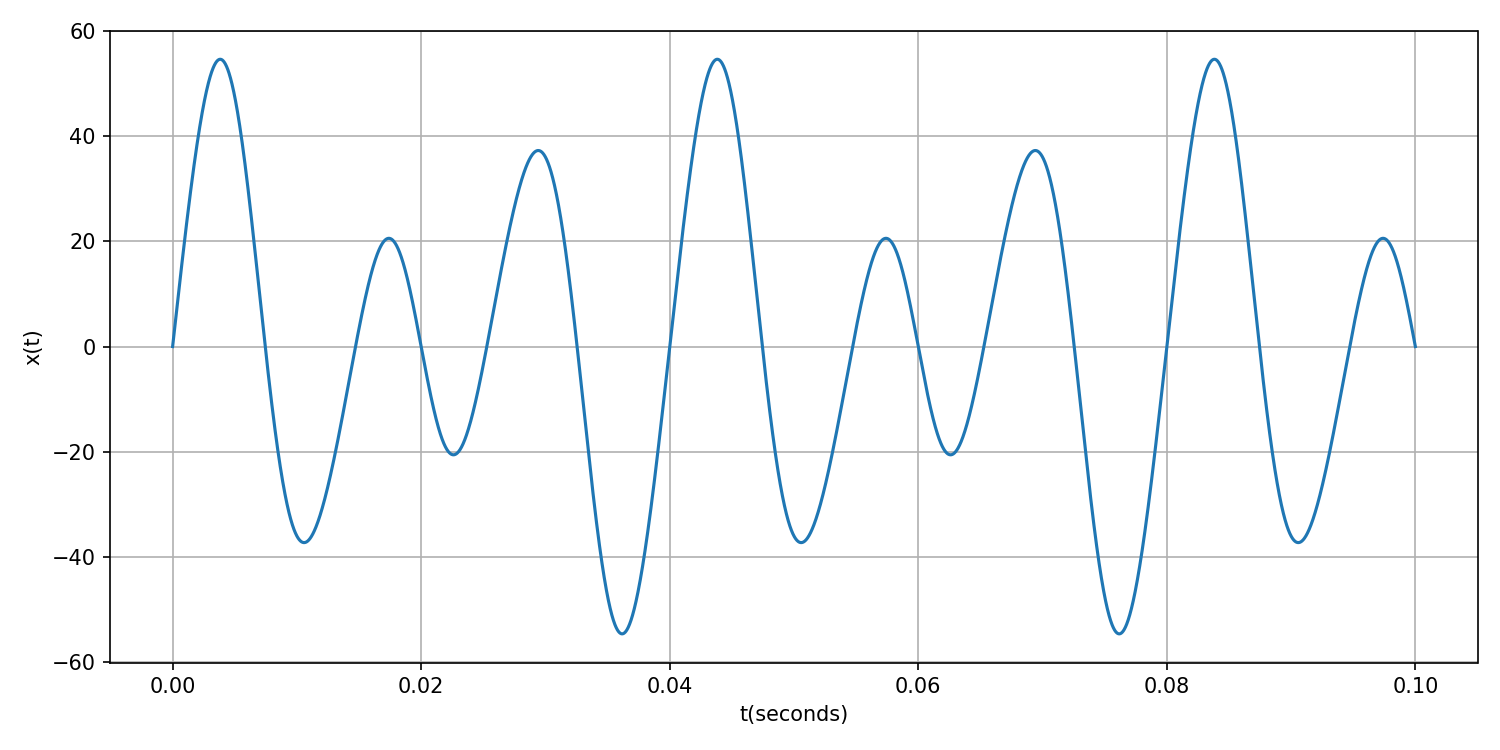
\includegraphics[width=1\textwidth]{figs/bm10.png}
    \caption{Plot of x(t) vs time}
    \label{plot of x(t) vs time}
\end{figure}

\text{The following code results in graph}
\begin{lstlisting}
Codes/bm10.py
\end{lstlisting}


% =========================================================
% QUESTION 11
% =========================================================



\item A voltage source $V_s = 5\sin\left(100t + \frac{\pi}{2}\right)\text{ volts}$ is driving a current $I = 10\sin\left(100t + \frac{\pi}{6}\right)\text{ mA}$ through a circuit. The average power dissipated in the circuit is \underline{\hspace{2cm}} $\text{mW}$.
\hfill \text{(GATE BM 2025)}

% =========================================================
% OPTIONS
% =========================================================
\begin{multicols}{2}
\begin{enumerate}
\setlength{\itemsep}{0pt}
    \item[(a)] $0.0$

    \item[(b)] $12.5$

    \item[(c)] $25.0$

    \item[(d)] $50.0$
\end{enumerate}
\end{multicols}

% =========================================================
% SOLUTION
% =========================================================

\solution

Given data from the problem:
\begin{align}
V_s(t) &= 5 \sin\left(100t + \frac{\pi}{2}\right) \text{ V} \\
I(t) &= 10 \sin\left(100t + \frac{\pi}{6}\right) \text{ mA}
\end{align}

Extracting the peak values and phase angles:
\begin{align}
V_0 &= 5 \text{ V}\\ I_0 &= 10 \text{ mA}\\
\phi_v &= \frac{\pi}{2} \text{ rad} \\
\phi_i &= \frac{\pi}{6} \text{ rad}
\end{align}

Calculate the phase difference $\theta$:
\begin{equation}
\theta = \phi_v - \phi_i = \frac{\pi}{2} - \frac{\pi}{6} = \frac{3\pi - \pi}{6} = \frac{2\pi}{6} = \frac{\pi}{3} \text{ rad}
\end{equation}
From \eqref{power}

Substituting these values into the average power formula:
\begin{align}
P_{\text{avg}} &= \frac{1}{2} \times 5 \times 10 \times \cos\left(\frac{\pi}{3}\right) \text{ mW} \\
P_{\text{avg}} &= 12.5 \text{ mW}
\end{align}


\begin{figure}[H]
    \centering
    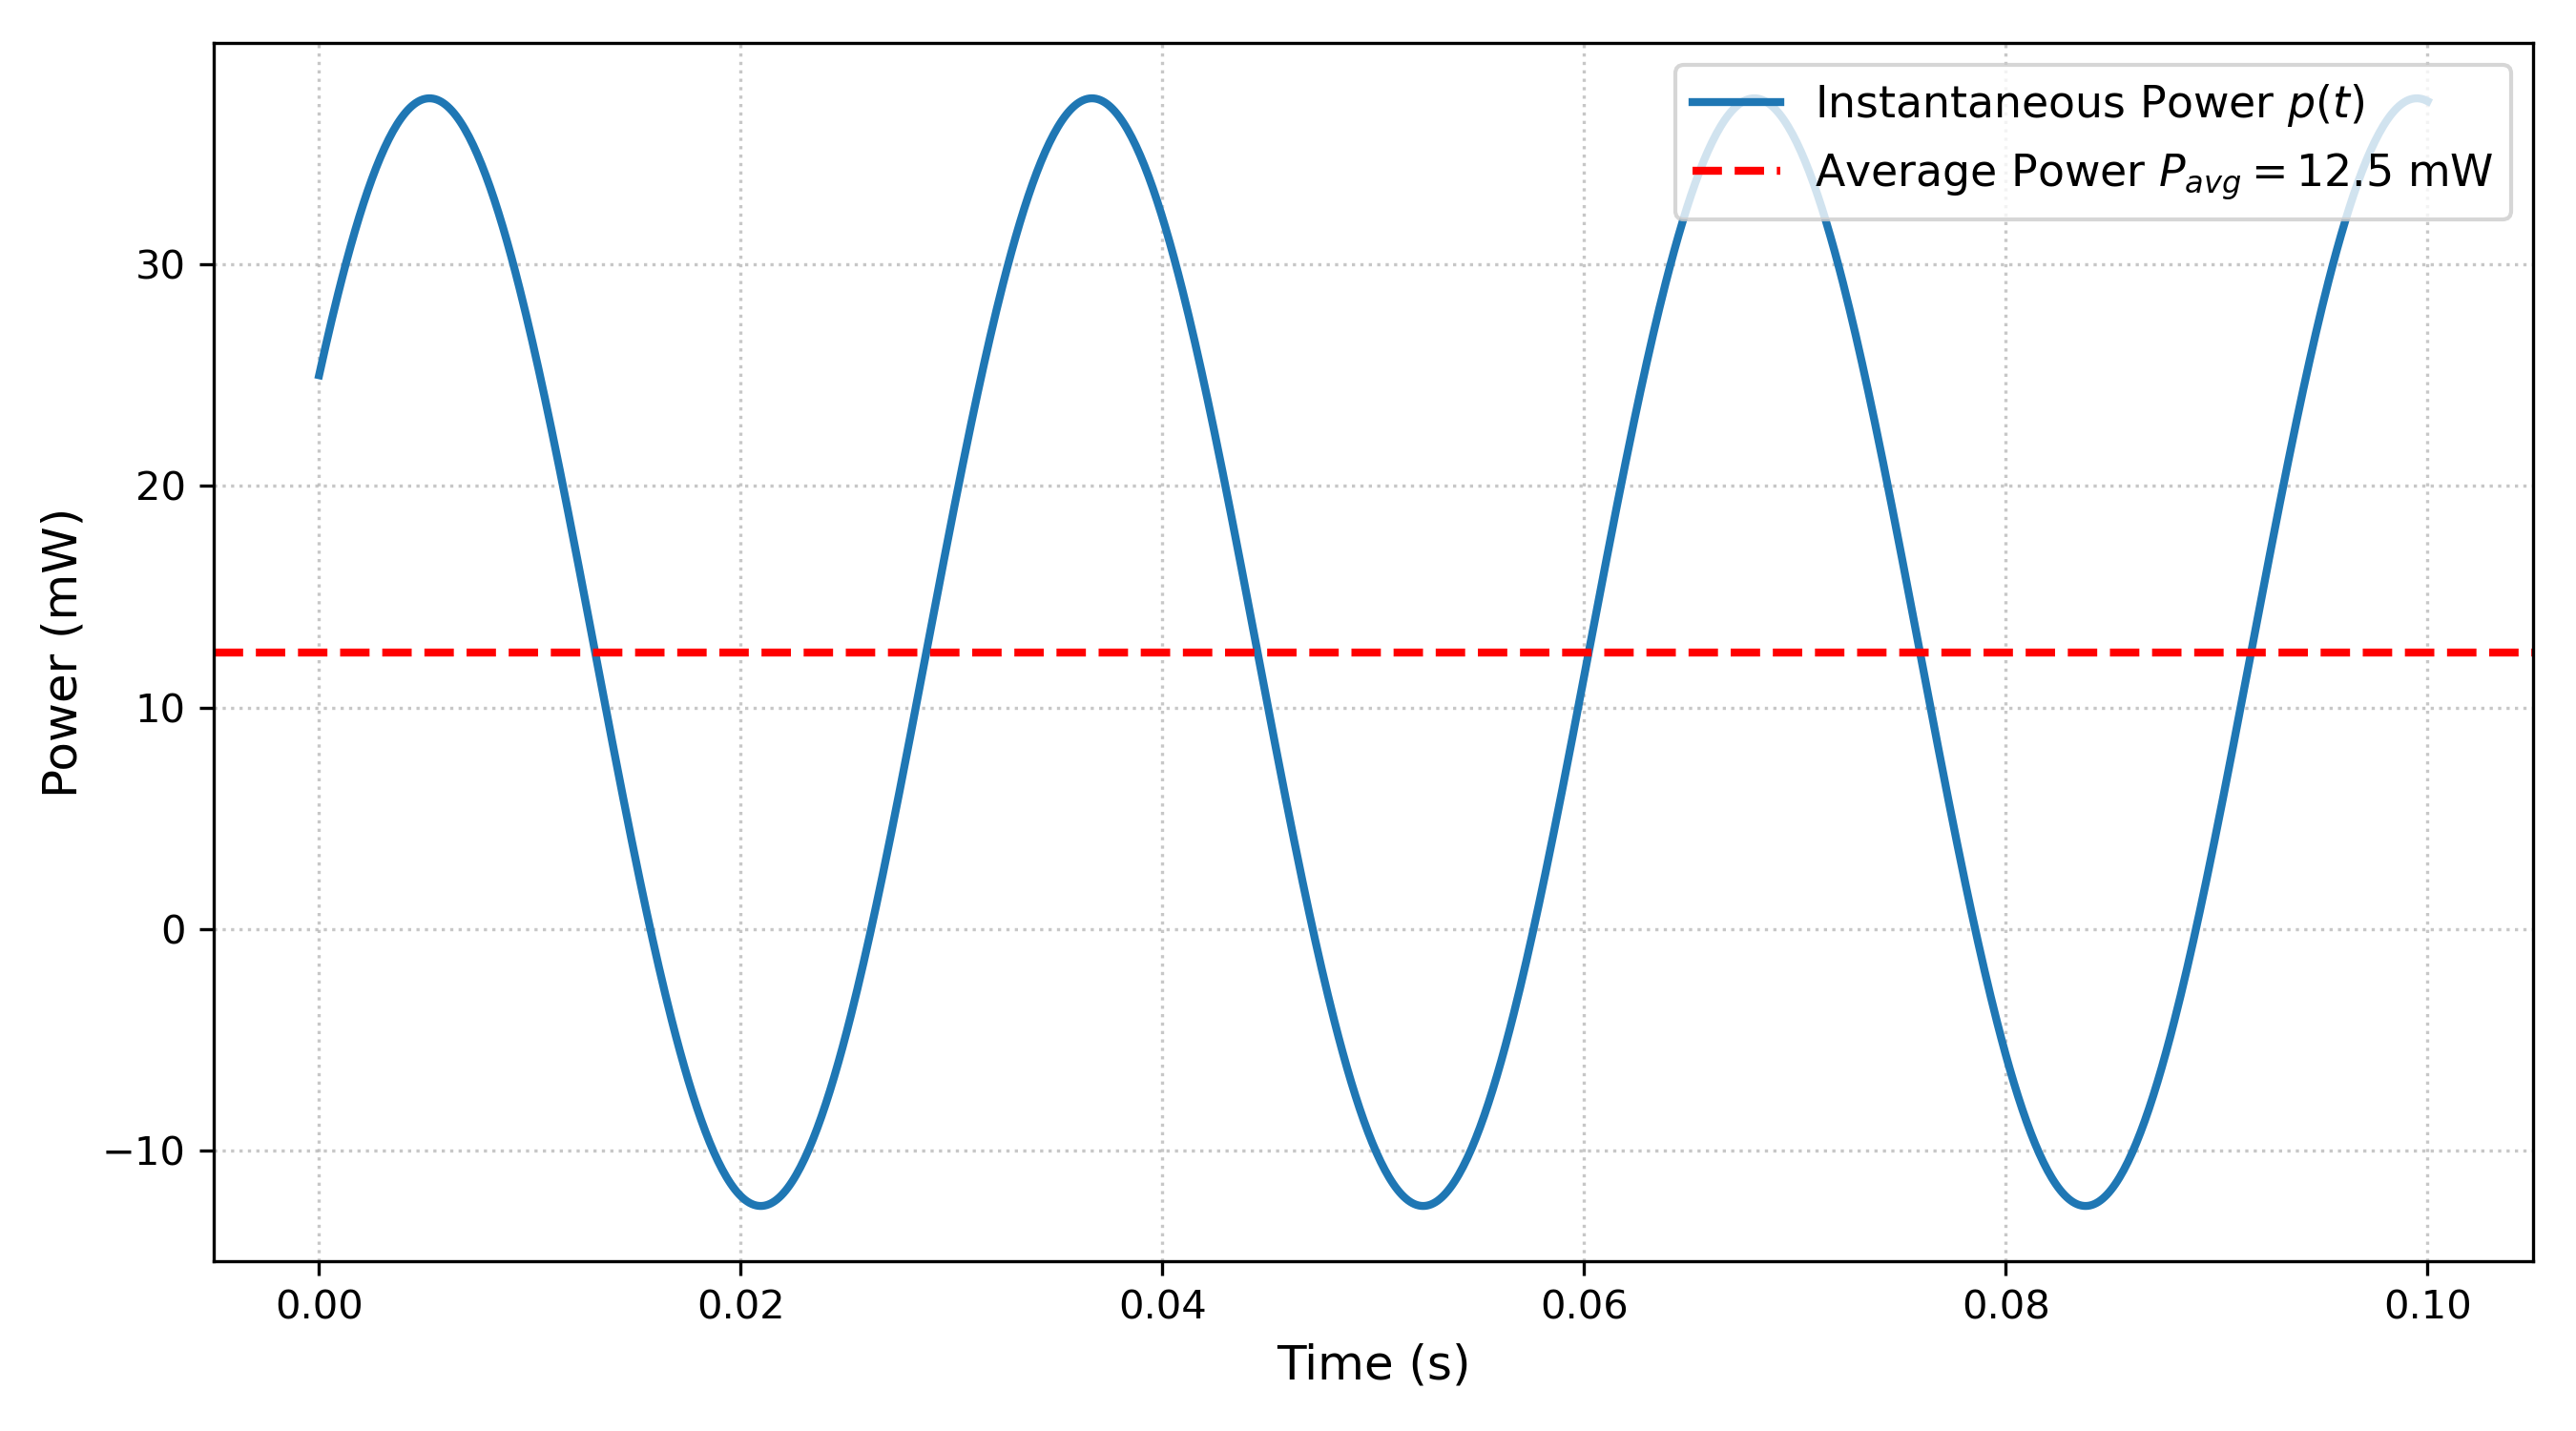
\includegraphics[width=0.75\textwidth]{figs/bm11.png}
    \caption{Power vs time}
    \label{power vs time}
\end{figure}

\text{The following code results the graph}
\begin{lstlisting}
Codes/bm11.py
\end{lstlisting}

% =========================================================
% QUESTION 12
% ========================================================

\item $N$ independent trials of a binomial random variable yield an expectation value of $16$ and variance of $12$. What is the value of $N$?
\hfill \text{(GATE BM 2025)}

% =========================================================
% OPTIONS
% =========================================================
\begin{multicols}{2}
\begin{enumerate}
\setlength{\itemsep}{0pt}
    \item[(a)] $80$

    \item[(b)] $60$

    \item[(c)] $45$

    \item[(d)] $64$
\end{enumerate}
\end{multicols}

% =========================================================
% SOLUTION
% =========================================================

\solution

For a Binomial distribution $X \sim \mathcal{B}(N, p)$ with $N$ independent trials and success probability $p$:

The expectation value (mean $\mu$) and variance ($\sigma^2$) are given by:
\begin{align}
\mu &= E(X) = Np = 16 \\
\sigma^2 &= \text{Var}(X) = Np(1 - p) = 12
\end{align}

From \eqref{gaussian}

Substituting the given mean $\mu = 16$ and variance $\sigma^2 = 12$:
\begin{align}
f_Y(x) = \frac{1}{\sqrt{24\pi}} \exp\left( -\frac{(x - 16)^2}{24} \right)
\end{align}

To find $N$, divide the variance equation by the mean equation:
From \eqref{variance}
\begin{align}
\frac{Np(1 - p)}{Np} = \frac{12}{16}
\end{align}

Simplifying:
\begin{align}
1 - p = \frac{3}{4} = 0.75
\end{align}

Solving for $p$:
\begin{align}
p = 1 - 0.75 = 0.25 = \frac{1}{4}
\end{align}

Substituting $p = \frac{1}{4}$ back into the expectation value equation:
\begin{align}
N \left(\frac{1}{4}\right) &= 16 \\
N &= 16 \times 4 \\
N &= 64
\end{align}


\begin{figure}[H]
    \centering
    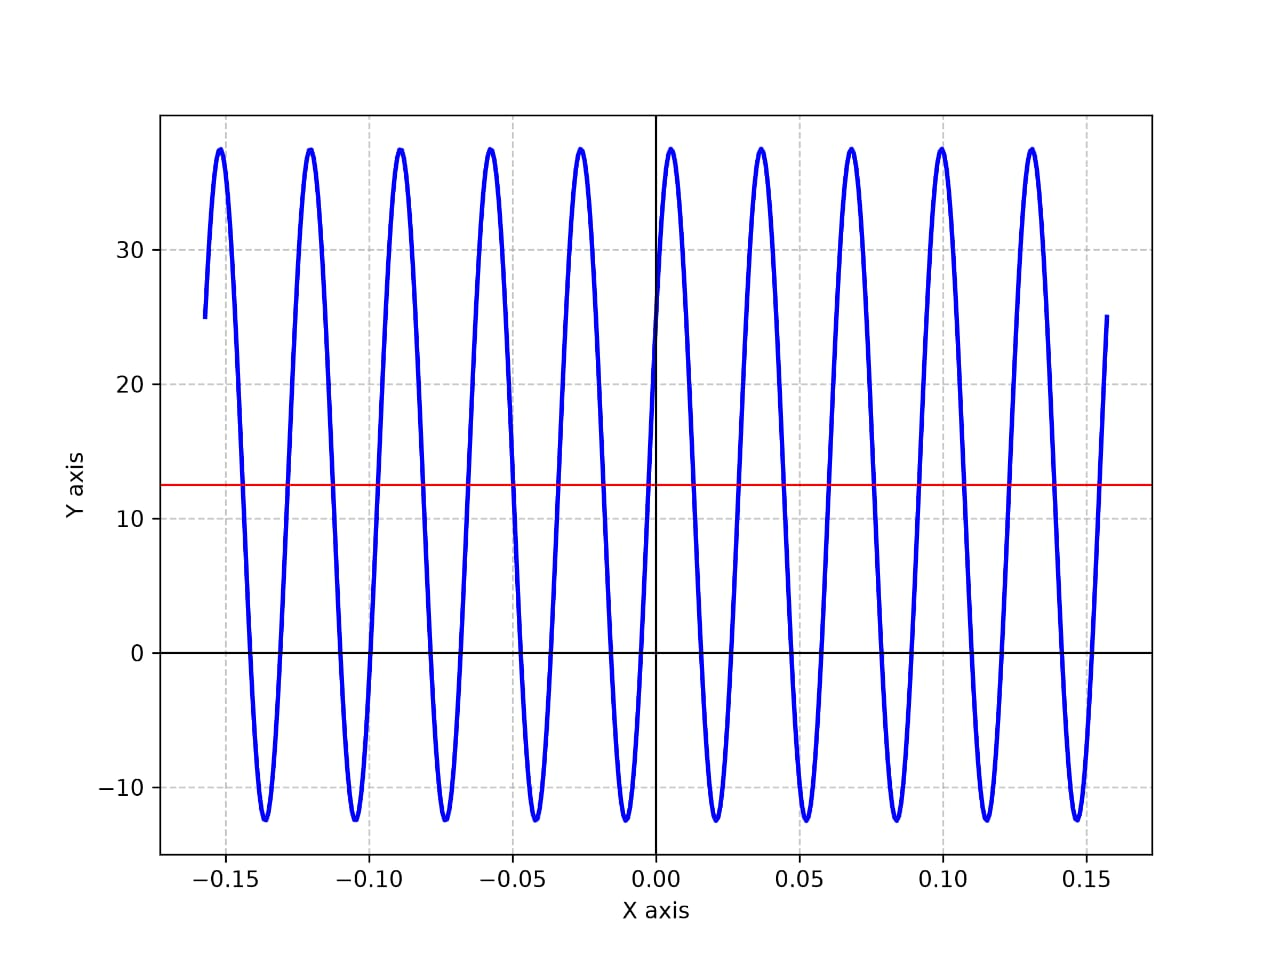
\includegraphics[width=0.75\textwidth]{figs/11.png}
    \caption{Probability vs values}
    \label{probability vs values}
\end{figure}

\text{The following code results the graph}
\begin{lstlisting}
Codes/bm12.py
\end{lstlisting}

% =========================================================
% QUESTION 13
% =========================================================

\item Given a function $y(x)$ satisfying the differential equation
\begin{align}
y'' - 0.25y = 0,
\end{align}
with initial conditions $y(0) = 1$; $y'(0) = 1$, what is the value of $y(\log_e 100)$?

Here, $y'$ and $y''$ are the first and second derivatives of $y$, respectively.
\hfill \text{(GATE BM 2025)}

% =========================================================
% OPTIONS
% =========================================================
\begin{multicols}{2}
\begin{enumerate}
\setlength{\itemsep}{0pt}
    \item[(a)] $14.05$

    \item[(b)] $14.25$

    \item[(c)] $14.95$

    \item[(d)] $14.65$
\end{enumerate}
\end{multicols}

% =========================================================
% SOLUTION
% =========================================================

\solution

Given the second-order linear differential equation:
\begin{equation}
y''(x) - 0.25 y(x) = 0
\end{equation}

with initial conditions $y(0) = 1$ and $y'(0) = 1$.


\text{Take the Laplace Transform on both sides}
Let $\mathcal{L}\{y(x)\} = Y(s)$. 
From \eqref{laplace}

Substituting into the differential equation gives:

\begin{align}
\left[ s^2 Y(s) - s y(0) - y'(0) \right] - 0.25 Y(s) = 0
\end{align}


\text{Substitute the initial conditions}
\
Substitute $y(0) = 1$ and $y'(0) = 1$:

\begin{align}
s^2 Y(s) - s - 1 - 0.25 Y(s) = 0
\end{align}

Group $Y(s)$ terms together as \eqref{partial}
\begin{align}
(s^2 - 0.25) Y(s) &= s + 1\\
Y(s) &= \frac{s + 1}{s^2 - 0.25}\\
&= \frac{s + 1}{\left(s - \frac{1}{2}\right)\left(s + \frac{1}{2}\right)}
\end{align}


\text{Apply Partial Fraction Decomposition}

Express $Y(s)$ as:
\begin{align}
Y(s) = \frac{A}{s - 0.5} + \frac{B}{s + 0.5}
\end{align}

Solving for constants $A$ and $B$:
\begin{align}
A &= \lim_{s \to 0.5} (s - 0.5) Y(s) \\
&= \frac{0.5 + 1}{0.5 + 0.5} = 1.5
\end{align}
\begin{align}
B &= \lim_{s \to -0.5} (s + 0.5) Y(s) \\
&= \frac{-0.5 + 1}{-0.5 - 0.5} = -0.5
\end{align}

So, the transform is:
\begin{align}
Y(s) = \frac{1.5}{s - 0.5} - \frac{0.5}{s + 0.5}
\end{align}


\text{Take the Inverse Laplace Transform}

Using $\mathcal{L}^{-1}\left\{\frac{1}{s - a}\right\} = e^{at}$:
\begin{align}
y(x) = 1.5 e^{0.5x} - 0.5 e^{-0.5x}
\end{align}


\text{Evaluate $y(\log_e 100)$}

Substitute $x = \log_e 100 = \ln(100)$:
\begin{align}
e^{0.5 \ln(100)} = e^{\ln(100^{0.5})} = \sqrt{100} = 10
\end{align}
\begin{align}
e^{-0.5 \ln(100)} = \frac{1}{\sqrt{100}} = \frac{1}{10} = 0.1
\end{align}

Now, evaluate $y(\ln 100)$:
\begin{align}
y(\ln 100) = 1.5(10) - 0.5(0.1) = 15 - 0.05 = 14.95
\end{align}
 

\begin{figure}[H]
    \centering
    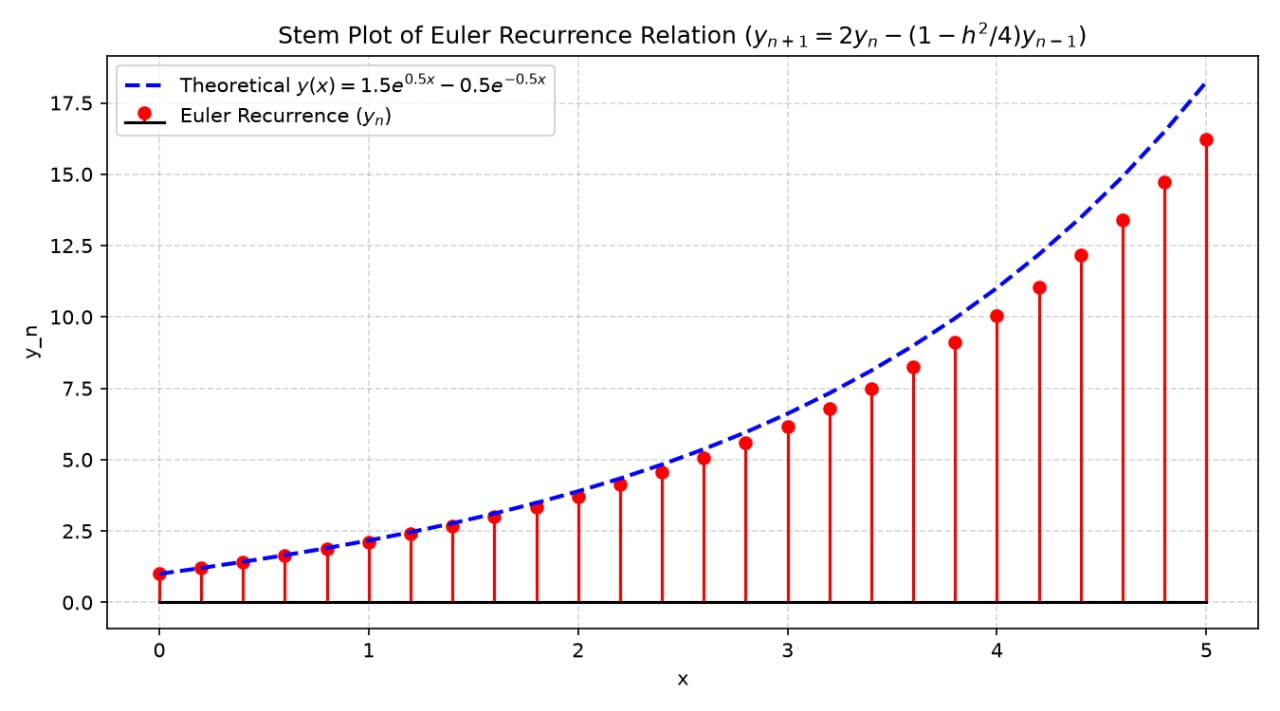
\includegraphics[width=1\textwidth]{figs/13.png}
    \caption{Stem plot of Euler Reccurrence relation}
    \label{Stem plot of Euler Reccurrence relation}
\end{figure}

\text{The following code results the 
}
\begin{lstlisting}
Codes/bm13.py
\end{lstlisting}

% =========================================================
% QUESTION 14
% =========================================================

\item In the circuit shown below, $V_{\text{in}} = 10\cos(1000t)\text{ volts}$. The magnitude of the input impedance of the circuit is 
\underline{\hspace{2cm}} $\text{k}\Omega$. (rounded off to one decimal place)

\begin{center}
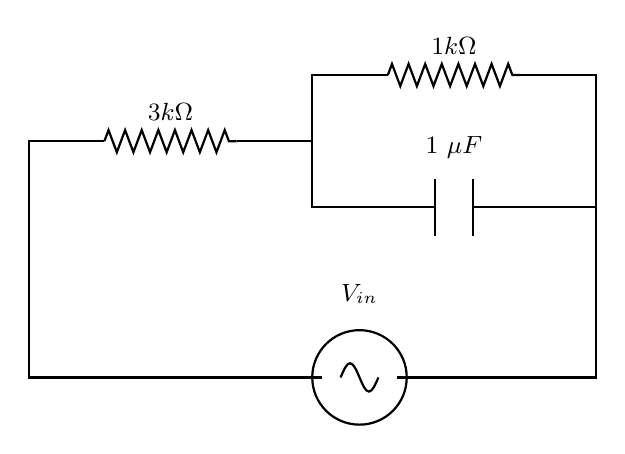
\begin{tikzpicture}[scale=1.2, every node/.style={font=\small}]

  % Top left wire & 3 k\Omega resistor
  \draw[thick] (0,-1) -- (0,1.5) -- (0.8,1.5);
  \draw[thick, decorate, decoration={zigzag, segment length=6pt, amplitude=4pt}] (0.8,1.5) -- (2.2,1.5);
  \node[above=4pt] at (1.5,1.5) {$3\text{ k}\Omega$};
  \draw[thick] (2.2,1.5) -- (3,1.5);
  
  % Parallel top branch: 1 k\Omega resistor
  \draw[thick] (3,1.5) -- (3,2.2) -- (3.8,2.2);
  \draw[thick, decorate, decoration={zigzag, segment length=6pt, amplitude=4pt}] (3.8,2.2) -- (5.2,2.2);
  \node[above=4pt] at (4.5,2.2) {$1\text{ k}\Omega$};
  \draw[thick] (5.2,2.2) -- (6,2.2) -- (6,1.5);
  
  % Parallel bottom branch: 1 \mu F capacitor
  \draw[thick] (3,1.5) -- (3,0.8) -- (4.3,0.8);
  \draw[thick] (4.3,0.5) -- (4.3,1.1);
  \draw[thick] (4.7,0.5) -- (4.7,1.1);
  \node[above=4pt] at (4.5,1.1) {$1\ \mu\text{F}$};
  \draw[thick] (4.7,0.8) -- (6,0.8);
  
  % Outer connections & AC Source
  \draw[thick] (6,1.5) -- (6,-1) -- (3.9,-1);
  \draw[thick] (0,0) -- (0,-1) -- (3.1,-1);
  \draw[thick] (3.5,-1) circle (0.5);
  \draw[thick] (3.3,-1) sin (3.4,-0.85) cos (3.5,-1) sin (3.6,-1.15) cos (3.7,-1);
  \node[above=6pt] at (3.5,-0.5) {$V_{\text{in}}$};
\end{tikzpicture}
\end{center}


\hfill \text{(GATE BM 2025)}

% =========================================================
% OPTIONS
% =========================================================
\begin{multicols}{2}
\begin{enumerate}
\setlength{\itemsep}{0pt}
    \item[(a)] $5.0$

    \item[(b)] $3.5$

    \item[(c)] $6.0$

    \item[(d)] $4.5$
\end{enumerate}
\end{multicols}


% =========================================================
% SOLUTION
% =========================================================

\solution

Given the input voltage $V_{\text{in}} = 10\cos(1000t)\text{ V}$, the circuit parameter values are:
\begin{align}
R_1 = 3\text{ k}\Omega, \quad R_2 = 1\text{ k}\Omega, \quad C = 1\,\mu\text{F}, \quad \omega = 1000\text{ rad/s}
\end{align}


Refer to \eqref{impedence deri}


Substituting $R_1$, $R_2$, $C$, and $\omega$: 

First calculate the normalized frequency factor:
\begin{align}
\omega R_2 C = (1000)(1 \times 10^3)(1 \times 10^{-6}) = 1
\end{align}

Now, compute real and imaginary components of $Z_p$:
\begin{align}
Z_p &= \frac{1 - j(1)}{1 + (1)^2}\\
&= 0.5 - j0.5\text{ k}\Omega
\end{align}

Total impedance:
\begin{align}
Z_{\text{in}} &= 3 + (0.5 - j0.5)\\
&= 3.5 - j0.5\text{ k}\Omega
\end{align}

Evaluating Magnitude $|Z_{\text{in}}|$:
\begin{align}
|Z_{\text{in}}| &= \sqrt{(3.5)^2 + (-0.5)^2} \\
&= \sqrt{12.25 + 0.25} \\
&= \sqrt{12.5} \\
&\approx 3.5\text{ k}\Omega
\end{align}

Evaluating Phase $\angle Z_{\text{in}}$:
\begin{align}
\angle Z_{\text{in}}\\
&= \tan^{-1}\left(\frac{-0.5}{3.5}\right)\\
&= -\tan^{-1}\left(\frac{1}{7}\right)\\
&\approx -8.13^\circ
\end{align}


\begin{figure}[H]
    \centering
    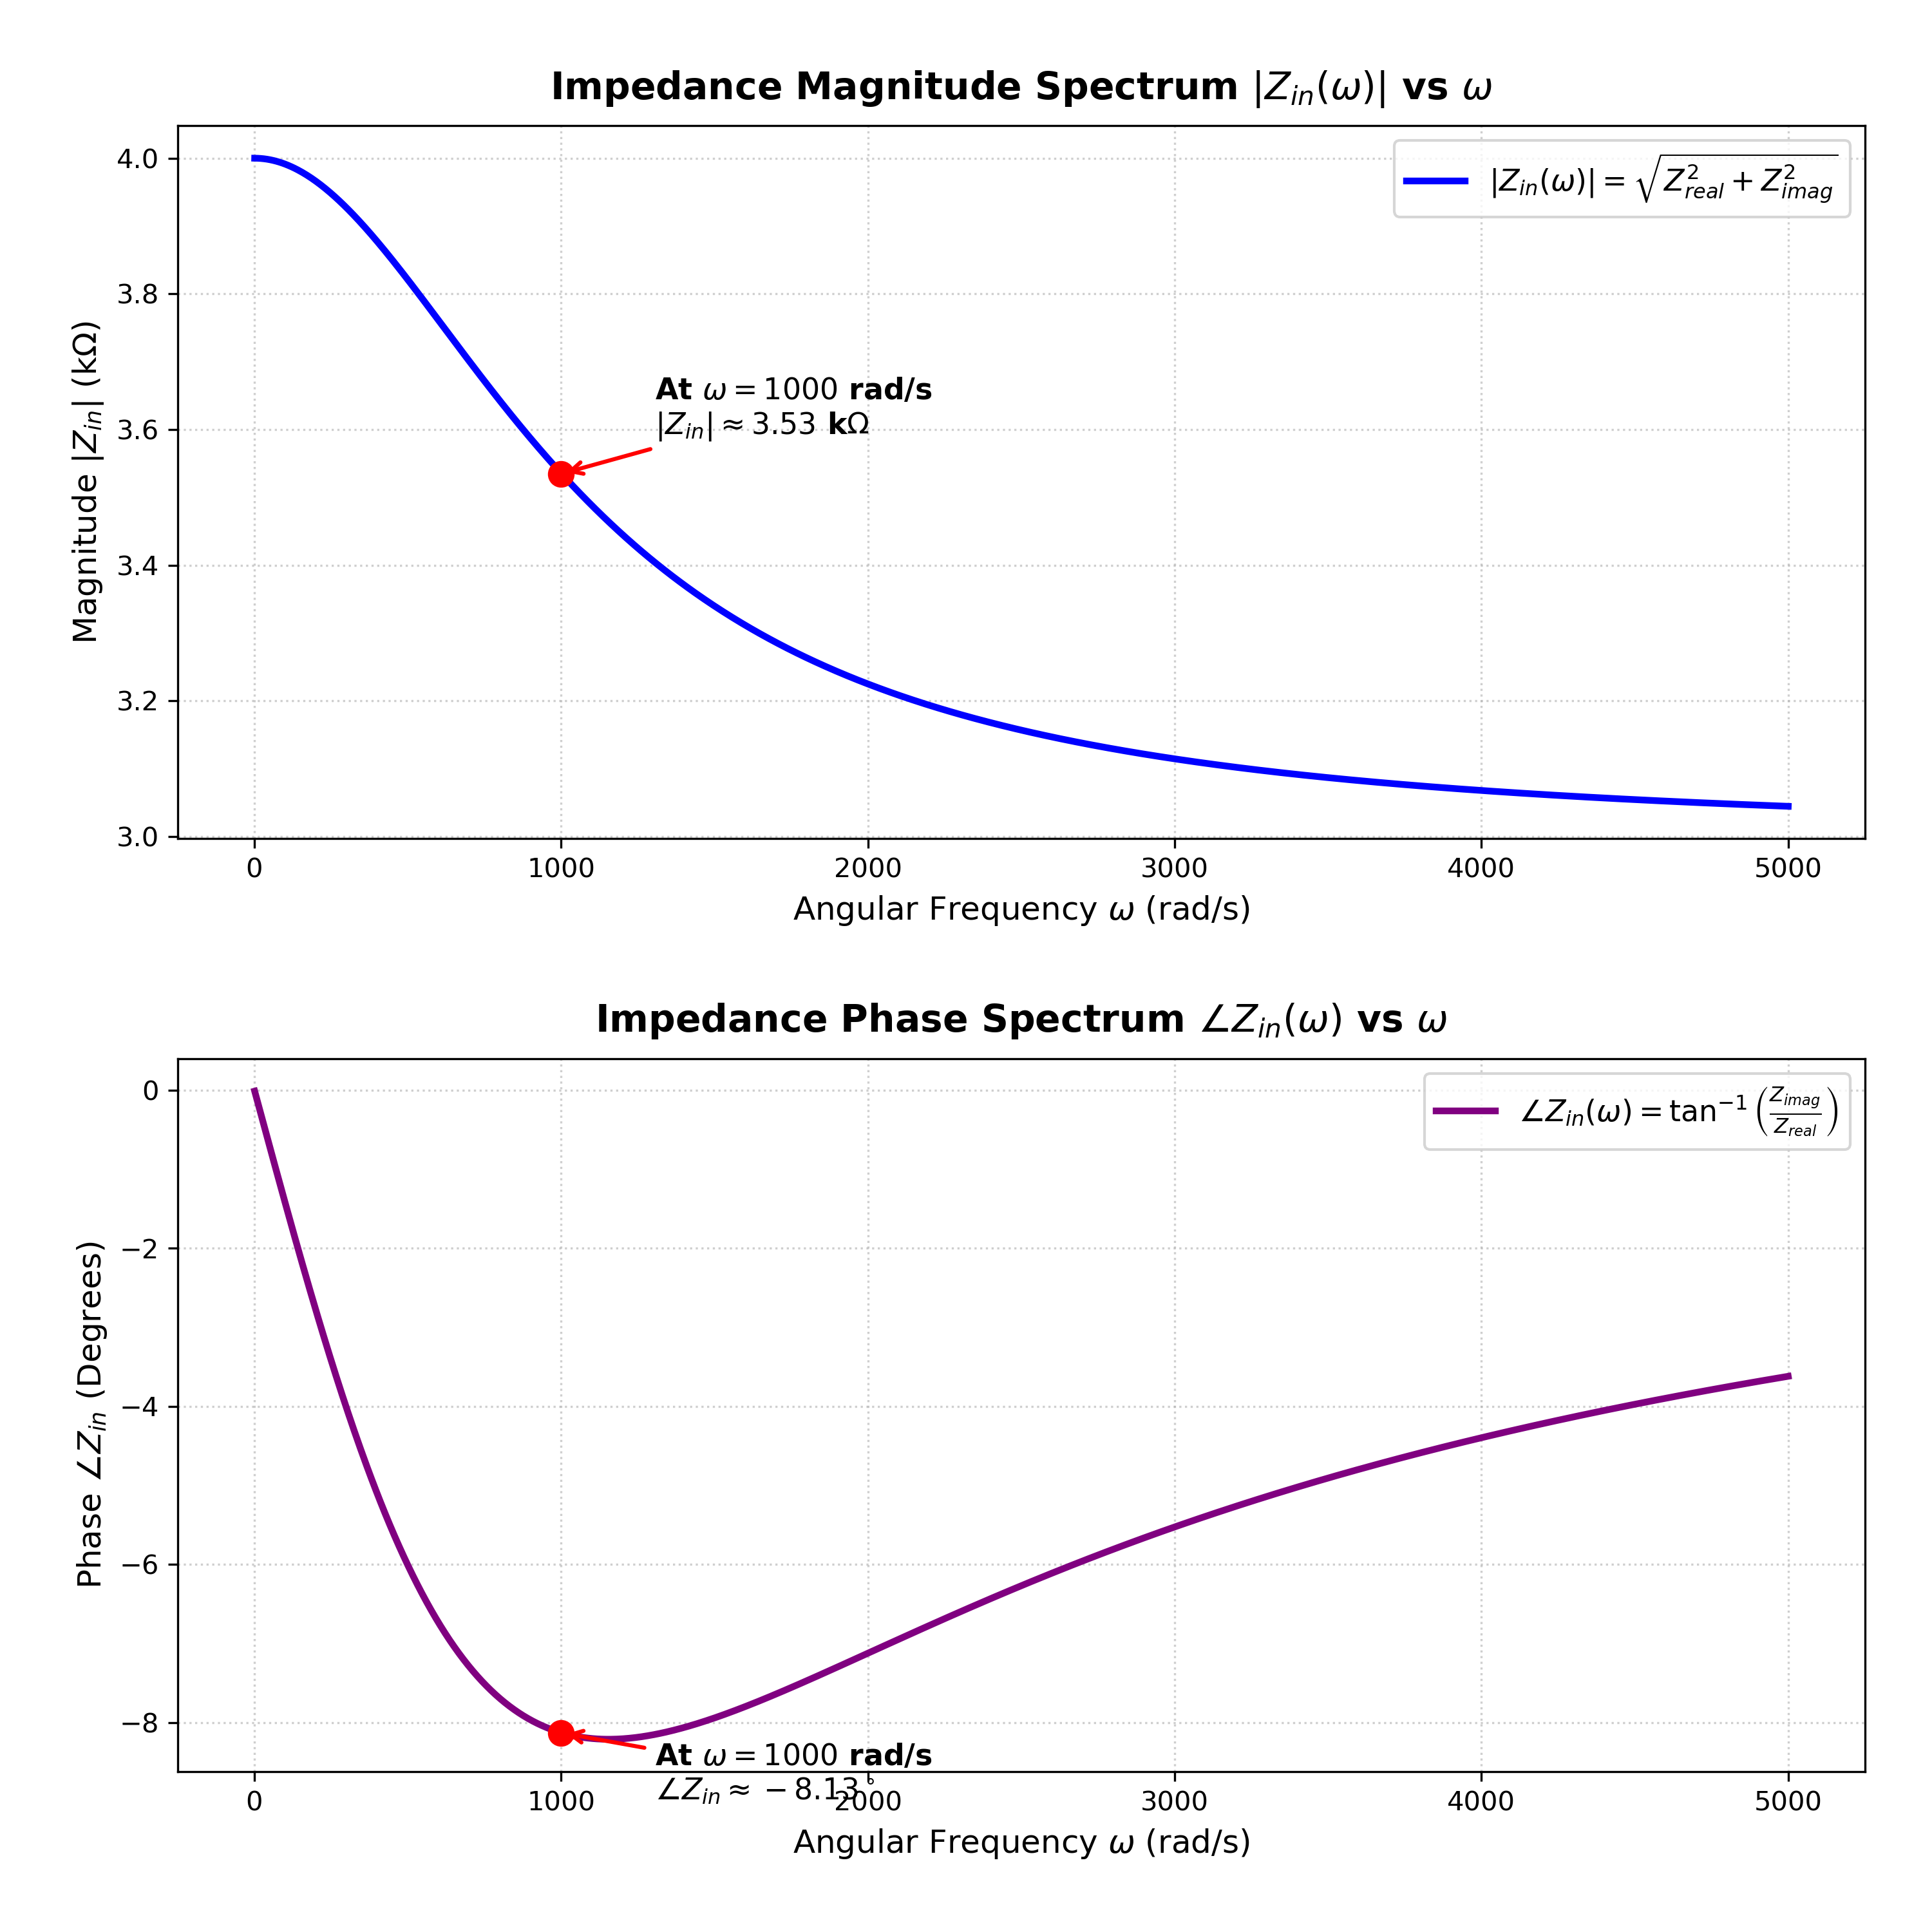
\includegraphics[width=1\textwidth]{figs/bm14.png}
    \caption{Impedance Magnitude VS Omega; Phase VS Omega}
    \label{Impedance Magnitude VS Omega; Phase VS Omega}
\end{figure}

\text{The following code results the graph}
\begin{lstlisting}
Codes/bm14.py
\end{lstlisting}

% =========================================================
% QUESTION 15
% =========================================================

\item Which of the following is/are CORRECT about the value of $y = \log_e(-e^x)$, where $x$ is a real number.
\hfill \text{(GATE BM 2025)}

% =========================================================
% OPTIONS
% =========================================================
\begin{multicols}{2}
\begin{enumerate}
\setlength{\itemsep}{0pt}
    \item[(a)] $y$ is real valued

    \item[(b)] $y$ is complex valued

    \item[(c)] $y = x \pm i n \pi$, where $n$ is an odd integer and $i = \sqrt{-1}$

    \item[(d)] $y = x \pm i n \pi$, where $n$ is an even integer and $i = \sqrt{-1}$
\end{enumerate}
\end{multicols}


% =========================================================
% SOLUTION
% =========================================================

\solution

Given the expression:

\begin{align}
y = \log_e(-e^x) = \ln(-e^x)
\end{align}

Using \eqref{log}

Taking the natural logarithm on both sides of \eqref{e^x}

\begin{align}
y = \ln\left(e^{x + i(2k+1)\pi}\right)
\end{align}

\begin{align}
y = x + i(2k+1)\pi, \quad \text{for } k \in \mathbb{Z}
\end{align}

Let $n = |2k + 1|$. Since $2k+1$ is always an odd integer, $n$ represents an odd integer:

\begin{align}
y = x \pm i n \pi, \quad \text{where } n \text{ is an odd integer and } i = \sqrt{-1}
\end{align}

Since $y$ contains an imaginary component $i n \pi$ (with $n \ge 1$), $y$ is a complex-valued function.

 Both statements (B) and (C) are correct.


                                          
% =========================================================
% QUESTION 16
% =========================================================

\item Two systems $U$ and $V$ are defined as shown below. Which of the following statement(s) is/are CORRECT?

\begin{center}
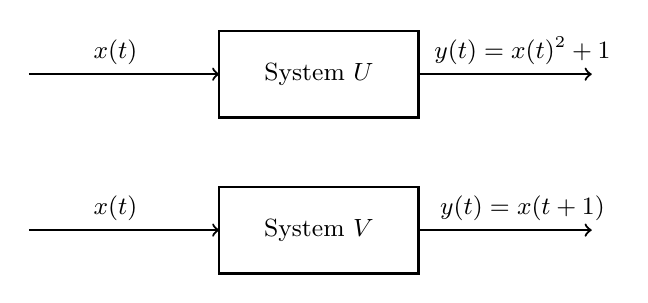
\begin{tikzpicture}[scale=1.1, every node/.style={font=\small}]

    % System U block and arrows
    \draw[thick] (0,1.8) -- (1.5,1.8);
    \draw[thick, ->] (1.5,1.8) -- (2.2,1.8);
    \node[above] at (1.0,1.8) {$x(t)$};

    \draw[thick] (2.2,1.3) rectangle (4.5,2.3);
    \node at (3.35,1.8) {System $U$};

    \draw[thick, ->] (4.5,1.8) -- (6.5,1.8);
    \node[above] at (5.7,1.8) {$y(t) = x(t)^2 + 1$};

    % System V block and arrows
    \draw[thick] (0,0) -- (1.5,0);
    \draw[thick, ->] (1.5,0) -- (2.2,0);
    \node[above] at (1.0,0) {$x(t)$};

    \draw[thick] (2.2,-0.5) rectangle (4.5,0.5);
    \node at (3.35,0) {System $V$};

    \draw[thick, ->] (4.5,0) -- (6.5,0);
    \node[above] at (5.7,0) {$y(t) = x(t + 1)$};

\end{tikzpicture}
\end{center}

\hfill \text{(GATE BM 2025)}

% =========================================================
% OPTIONS
% =========================================================
\begin{multicols}{2}
\begin{enumerate}
\setlength{\itemsep}{0pt}
    \item[(a)] System $U$ is nonlinear; System $V$ is linear

    \item[(b)] System $U$ is causal; System $V$ is noncausal

    \item[(c)] System $U$ is noncausal; System $V$ is causal

    \item[(d)] System $U$ is nonlinear; System $V$ is nonlinear
\end{enumerate}
\end{multicols}

% =========================================================
% SOLUTION
% =========================================================
\solution


\text Conditions to be Satisfied are \eqref{conditions}

\text System U
\begin{equation}
y(t) = x(t)^2 + 1
\end{equation}

Linearity check:
\begin{align}
T\{a \cdot x(t)\} &= [a \cdot x(t)]^2 + 1 \\
&= a^2 x(t)^2 + 1 \\
&\neq a \cdot [x(t)^2 + 1]
\end{align}
System U is nonlinear.

Causality check:
\begin{equation}
y(t) \text{ depends only on } x(t) \text{ at time } t
\end{equation}
System U is causal.

\text System V
\begin{equation}
y(t) = x(t + 1)
\end{equation}

Linearity check:
\begin{align}
T\{a \cdot x_1(t) + b \cdot x_2(t)\} &= a \cdot x_1(t + 1) + b \cdot x_2(t + 1) \\
&= a \cdot y_1(t) + b \cdot y_2(t)
\end{align}
System V is linear.

Causality check:
\begin{align}
\text{At } t = 0: \quad y(0) = x(1)
\end{align}
Since $y(0)$ depends on the future input $x(1)$, System V is noncausal.




% =========================================================
% QUESTION 17
% =========================================================

\item A discrete linear time invariant system has an impulse response function given by
\begin{align}
h(n) = \delta(n) + \frac{1}{2}\delta(n-1) + \frac{1}{3}\delta(n-2).
\end{align}
For input signal $x(n) = \delta(n) + \delta(n-1)$, which of the following option(s) is/are CORRECT for the output signal $y(n)$?
\hfill \text{(GATE BM 2025)}

% =========================================================
% OPTIONS
% =========================================================
\begin{multicols}{2}
\begin{enumerate}
\setlength{\itemsep}{0pt}
    \item[(a)] $y(2) = 11/6$

    \item[(b)] $y(2) = 5/6$

    \item[(c)] $y(2) = 0$ for all $k \ge 3$

    \item[(d)] $y(2) = 0$ for all $k \ge 4$
\end{enumerate}
\end{multicols}

% =========================================================
% SOLUTION
% =========================================================

\solution


\text{Express sequences in vector form}

The impulse response sequence $h(n)$ of length $M = 3$ is:

\begin{align}
	\vec{h(n)}=\myvec{1 & 1/2 & 1/3}
\end{align}

The input signal sequence $x(n)$ of length $N = 2$ is:

\begin{align}
	\vec{x(n)}=\myvec{1 & 1}
\end{align}
The linear convolution $y(n) = h(n) * x(n)$ has a total length of $4$ points (spanning $n = 0, 1, 2, 3$). (From \eqref{convolution})

\text{Construct the Convolution (Toeplitz) Matrix}
Linear convolution can be represented as a matrix-vector product $\vec{y}$ = $\vec{H}$ $\vec{x}$, where $\vec{H}$ is a (M+N-1)*N=8 lower-triangular Toeplitz matrix formed by shifting $h(n)$ downwards:
\begin{align}
 \vec{H}=\myvec{ 
   h(0) & 0 \\ 
   h(1) & h(0) \\ 
   h(2) & h(1) \\ 
   0 & h(2) 
   }
\end{align} 
\begin{align}
  =\myvec{ 
    1 & 0 \\ 
    1/2 & 1 \\
    1/3 & 1/2 \\
    0 & 1/3 
    }
    \end{align}
The input vector $\vec{x}$ is:
\begin{align}
 \vec{x}=\myvec{
          x(0) \\
          x(1)
          }
          =\myvec{
          1\\
          1
          }
\end{align}

\text{Matrix-Vector Multiplication}
\begin{align}
	\myvec{
	y(0) \\
	y(1) \\
	y(2) \\
	y(3)
	}=
	\myvec{
	1 & 0 \\
	1/2 & 1 \\
	1/3 & 1/2 \\
	0 & 1/3 
	}
	\myvec{
	1 \\
	1
	}
\end{align}

Computing each element:
\begin{align}
y(0) = 1(1) + 0(1) = 1\\
y(1) = \frac{1}{2}(1) + 1(1) = \frac{3}{2}\\
y(2) = \frac{1}{3}(1) + \frac{1}{2}(1) = \frac{5}{6}\\
y(3) = 0(1) + \frac{1}{3}(1) = \frac{1}{3}
\end{align}
For $k \ge 4$, $y(k) = 0$ since the signal duration ends at $n = 3$.

\text{Verify the Options}
\begin{itemize}
  \item \text{Option (a):} $y(2) = \frac{11}{6}$ \quad (\text{Incorrect})
  \item \text{Option (b):} $y(2) = \frac{5}{6}$ \quad (\text{Correct})
  \item \text{Option (c):} $y(k) = 0$ for all $k \ge 3$ \quad (\text{Incorrect, since } $y(3) = \frac{1}{3} \neq 0$)
  \item \text{Option (d):} $y(k) = 0$ for all $k \ge 4$ \quad (\text{Correct})
\end{itemize}

\begin{figure}[H]
    \centering
    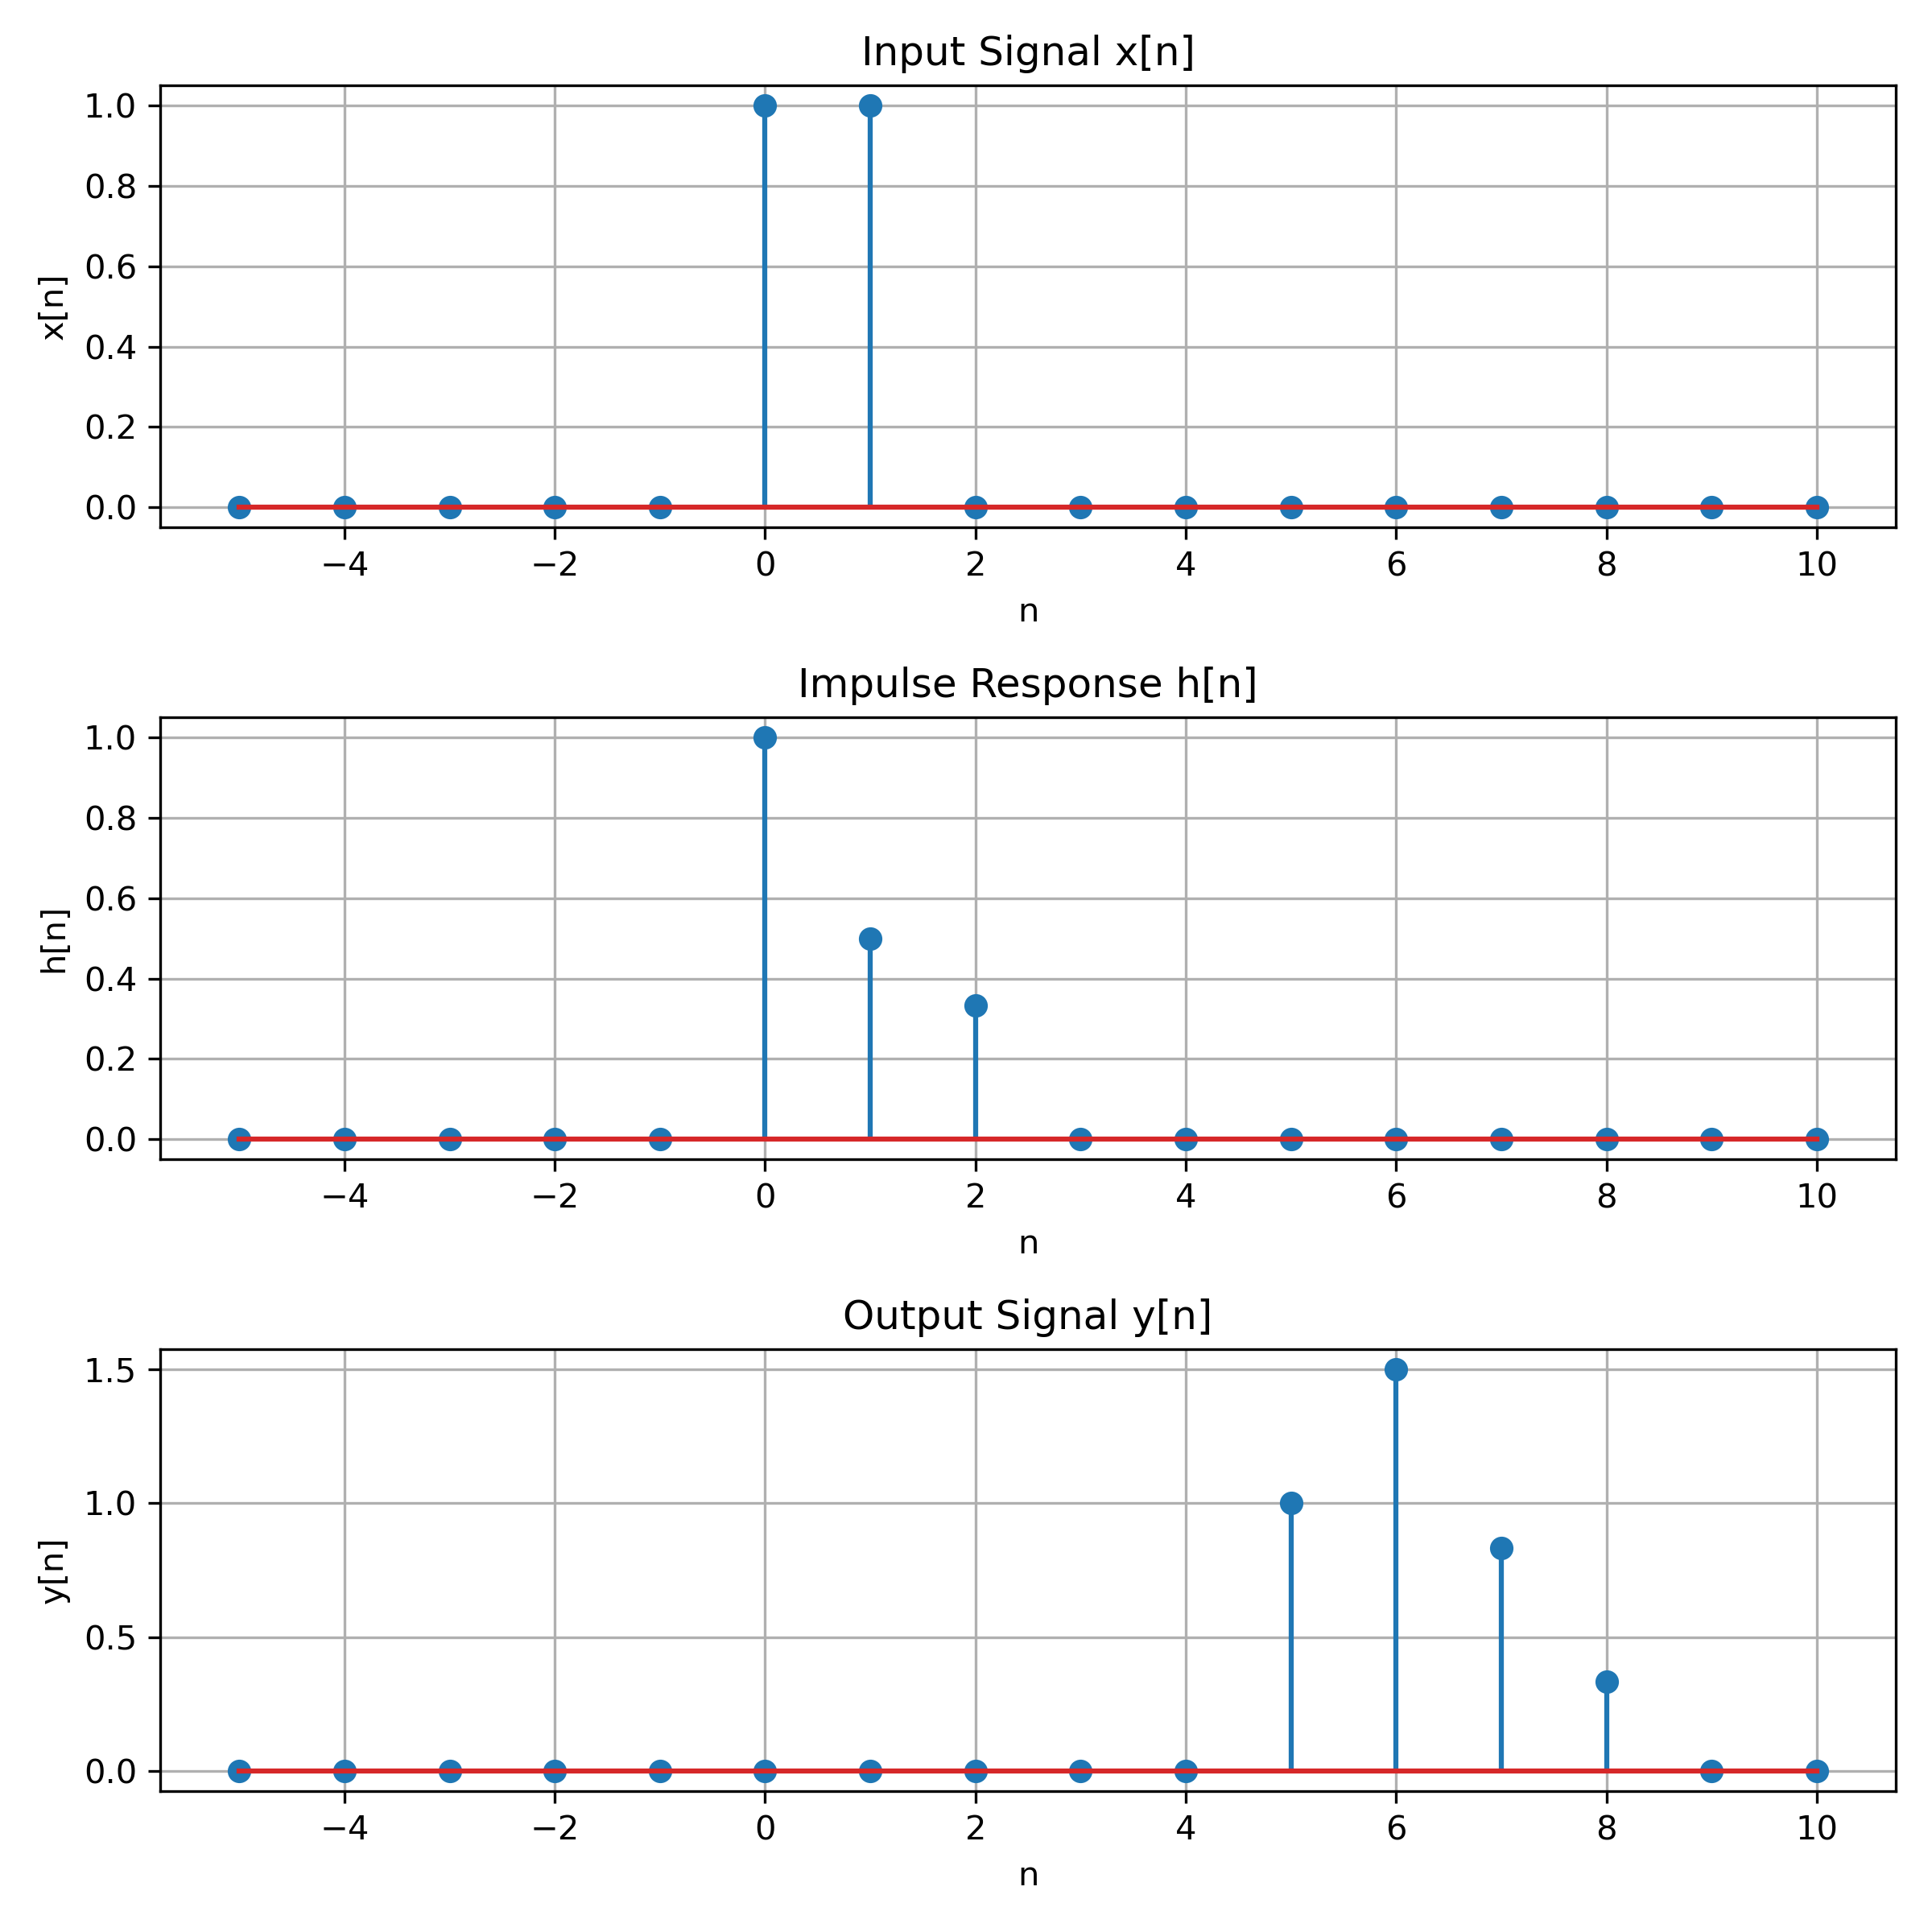
\includegraphics[width=1\textwidth]{figs/bm17a.png}
    \caption{x[n],h[n],y[n] vs n}
    \label{signals vs n}
\end{figure}

\text{The following code results the graph}
\begin{lstlisting}
Codes/bm17a.py
\end{lstlisting}


% =========================================================
% QUESTION 18
% =========================================================

\item For an 8-bit Digital to Analog Converter (DAC), the binary input 0000 0000 results in $0\text{ V}$, and 1111 1111 results in $5\text{ V}$. The output of the DAC for an input of 1011 0111 is \underline{\hspace{2cm}} (in volts, rounded off to two decimal places).
\hfill \text{(GATE BM 2025)}

% =========================================================
% SOLUTION
% =========================================================

\solution

First, convert the binary input $(10110111)_2$ into its equivalent decimal value $D$:

\begin{align}
D = 1 \cdot 2^7 + 0 \cdot 2^6 + 1 \cdot 2^5 + 1 \cdot 2^4 + 0 \cdot 2^3 + 1 \cdot 2^2 + 1 \cdot 2^1 + 1 \cdot 2^0
\end{align}

\begin{align}
D = 128 + 0 + 32 + 16 + 0 + 4 + 2 + 1 = 183
\end{align}

For an 8-bit DAC:
\begin{itemize}
    \item Minimum digital value $(00000000)_2 = 0$ corresponds to $0\text{ V}$.
    \item Maximum digital value $(11111111)_2 = 255$ corresponds to Full-Scale Voltage $V_{\text{FS}} = 5\text{ V}$.
\end{itemize}

From \eqref{output}
where $n = 8$ bits, so $2^8 - 1 = 255$.

Substituting $D = 183$ and $V_{\text{FS}} = 5\text{ V}$:

\begin{align}
V_{\text{out}} = 5 \times \left( \frac{183}{255} \right)
\end{align}

\begin{align}
V_{\text{out}} = \frac{915}{255} \approx 3.5882\text{ V}
\end{align}

Rounding off to two decimal places gives: 3.59

\text{The following code verifies the answer}
\begin{lstlisting}
Codes/bm18.py
\end{lstlisting}


% =========================================================
% QUESTION 19
% =========================================================

\item What is the output voltage Vout for the circuit shown below? \underline{\hspace{2cm}} (in volts, rounded off to the nearest integer).

\begin{center}
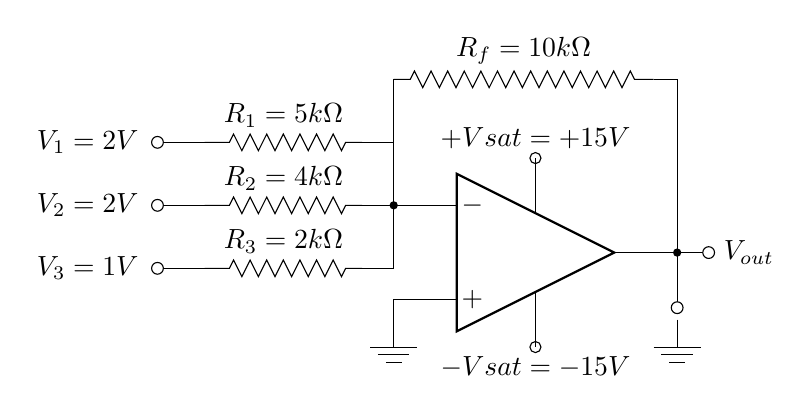
\begin{tikzpicture}[
    % Define custom styles using TikZ native features
    resistor/.style={
        circuitikz/resistor style/.style={},
        decorate, 
        decoration={zigzag, segment length=6pt, amplitude=3pt, pre length=6pt, post length=6pt}
    },
    terminal/.style={circle, draw, inner sep=1.5pt, fill=white},
    dot/.style={circle, fill, inner sep=1.2pt}
]

  % 1. Draw Op-Amp Triangle
  \draw[thick] (0,0) -- (0,2) -- (2,1) -- cycle;
  
  % Input Labels inside triangle (+ on bottom, - on top)
  \node at (0.2, 1.6) {$-$};
  \node at (0.2, 0.4) {$+$};

  % 2. Power Supply Lines
  \draw (1, 1.5) -- (1, 2.2) node[above] {$+\text{Vsat} = +15\text{ V}$};
  \draw (1, 2.2) circle (2pt);
  
  \draw (1, 0.5) -- (1, -0.2) node[below] {$-\text{Vsat} = -15\text{ V}$};
  \draw (1, -0.2) circle (2pt);

  % 3. Non-Inverting Input (+) Ground Connection
  \draw (0, 0.4) -- (-0.8, 0.4) -- (-0.8, -0.2);
  % Ground Symbol
  \draw (-1.1, -0.2) -- (-0.5, -0.2);
  \draw (-1.0, -0.3) -- (-0.6, -0.3);
  \draw (-0.9, -0.4) -- (-0.7, -0.4);

  % 4. Inverting Input (-) Node
  \draw (0, 1.6) -- (-0.8, 1.6) coordinate (invNode);
  \fill (-0.8, 1.6) circle (1.5pt);

  % 5. Three Input Resistors (R1, R2, R3)
  % R1 (Top)
  \draw (invNode) |- (-1.2, 2.4);
  \draw[resistor] (-1.2, 2.4) -- (-3.2, 2.4) node[midway, above=2pt] {$R_1 = 5\text{ k}\Omega$};
  \draw (-3.2, 2.4) -- (-3.8, 2.4) node[terminal] {} node[left] {$V_1 = 2\text{ V}\ $};

  % R2 (Middle)
  \draw (invNode) -- (-1.2, 1.6);
  \draw[resistor] (-1.2, 1.6) -- (-3.2, 1.6) node[midway, above=2pt] {$R_2 = 4\text{ k}\Omega$};
  \draw (-3.2, 1.6) -- (-3.8, 1.6) node[terminal] {} node[left] {$V_2 = 2\text{ V}\ $};

  % R3 (Bottom)
  \draw (invNode) |- (-1.2, 0.8);
  \draw[resistor] (-1.2, 0.8) -- (-3.2, 0.8) node[midway, above=2pt] {$R_3 = 2\text{ k}\Omega$};
  \draw (-3.2, 0.8) -- (-3.8, 0.8) node[terminal] {} node[left] {$V_3 = 1\text{ V}\ $};

  % 6. Feedback Resistor (Rf)
  \draw (invNode) -- (-0.8, 3.2);
  \draw[resistor] (-0.8, 3.2) -- (2.5, 3.2) node[midway, above=2pt] {$R_f = 10\text{ k}\Omega$};
  \draw (2.5, 3.2) -| (2.8, 1.0);

  % 7. Output Line and Terminal
  \draw (2, 1) -- (3.2, 1) node[terminal] {} node[right=2pt] {$V_{\text{out}}$};
  \fill (2.8, 1) circle (1.5pt);

  % Ground at Output Terminal
  \draw (2.8, 1) -- (2.8, 0.3) node[terminal] {};
  \draw (2.8, 0.15) -- (2.8, -0.2);
  % Ground Symbol
  \draw (2.5, -0.2) -- (3.1, -0.2);
  \draw (2.6, -0.3) -- (3.0, -0.3);
  \draw (2.7, -0.4) -- (2.9, -0.4);

\end{tikzpicture}
\end{center}

\hfill \text{(GATE BM 2025)}

% =========================================================
% SOLUTION
% =========================================================

\solution

The given operational amplifier circuit is an inverting summing amplifier. 

\text Given:
\begin{itemize}
    \item $R_f = 10\text{ k}\Omega$
    \item $R_1 = 5\text{ k}\Omega, \quad V_1 = 2\text{ V}$
    \item $R_2 = 4\text{ k}\Omega, \quad V_2 = 2\text{ V}$
    \item $R_3 = 2\text{ k}\Omega, \quad V_3 = 1\text{ V}$
    \item Power supply saturation limits: $\pm V_{\text{sat}} = \pm 15\text{ V}$
\end{itemize}

Substitute the given component values into \eqref{amplifier}

\begin{align}
V_{\text{out}} = -\left( \frac{10}{5}(2) + \frac{10}{4}(2) + \frac{10}{2}(1) \right)
\end{align}

\begin{align}
V_{\text{out}} = -\left( 2(2) + 2.5(2) + 5(1) \right)
\end{align}

\begin{align}
V_{\text{out}} = -(4 + 5 + 5) = -14\text{ V}
\end{align}

Since the calculated voltage ($-14\text{ V}$) lies within the saturation limits ($-15\text{ V}$ to $+15\text{ V}$), the op-amp stays in its linear region.


% =========================================================
% QUESTION 20
% =========================================================


\item The frequency of the oscillator circuit shown in the figure below is \underline{\hspace{2cm}} $\text{kHz}$. (rounded off to two decimal places)

Given: $R = 1\text{ k}\Omega$; $R_1 = 2\text{ k}\Omega$; $R_2 = 6\text{ k}\Omega$; $C = 0.1\ \mu\text{F}$

\begin{center}
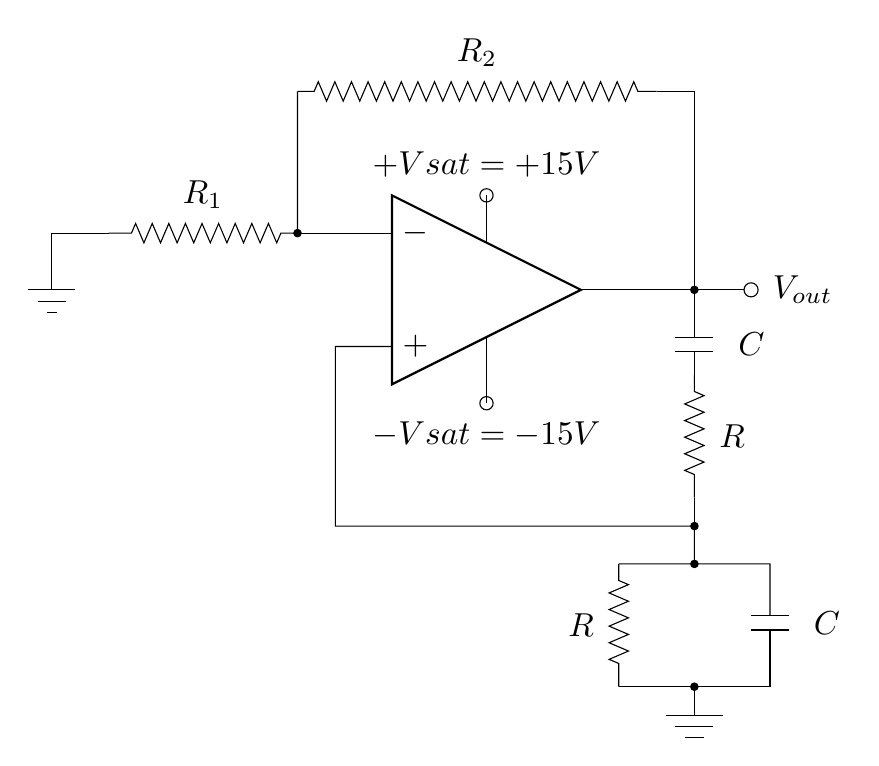
\begin{tikzpicture}[
    scale=1.2, transform shape,
    resistor/.style={
        decorate, 
        decoration={zigzag, segment length=6pt, amplitude=3.5pt, pre length=6pt, post length=6pt}
    },
    terminal/.style={circle, draw, inner sep=1.5pt, fill=white},
    dot/.style={circle, fill, inner sep=1.3pt}
]

  % 1. Op-Amp Triangle
  \draw[thick] (0,0) -- (0,2) -- (2,1) -- cycle;
  
  % Input Labels (- on top, + on bottom)
  \node at (0.25, 1.6) {$-$};
  \node at (0.25, 0.4) {$+$};

  % 2. Power Supply Connections (Moved outward for spacing)
  \draw (1, 1.5) -- (1, 2.0) node[above=2pt] {$+\text{Vsat} = +15\text{ V}$};
  \draw (1, 2.0) circle (2pt);
  
  \draw (1, 0.5) -- (1, -0.2) node[below=2pt] {$-\text{Vsat} = -15\text{ V}$};
  \draw (1, -0.2) circle (2pt);

  % 3. Inverting Input (-) Branch: R1 to Ground
  \draw (0, 1.6) -- (-1.0, 1.6) coordinate (invNode);
  \fill (invNode) circle (1.3pt);
  
  \draw[resistor] (invNode) -- (-3.0, 1.6) node[midway, above=4pt] {$R_1$};
  \draw (-3.0, 1.6) -- (-3.6, 1.6) -- (-3.6, 1.0);
  % Ground Symbol for R1
  \draw (-3.85, 1.0) -- (-3.35, 1.0);
  \draw (-3.75, 0.88) -- (-3.45, 0.88);
  \draw (-3.65, 0.76) -- (-3.55, 0.76);

  % 4. Feedback Resistor R2 (Higher elevation to avoid +Vsat label)
  \draw (invNode) -- (-1.0, 3.1);
  \draw[resistor] (-1.0, 3.1) -- (2.8, 3.1) node[midway, above=4pt] {$R_2$};
  \draw (2.8, 3.1) -| (3.2, 1.0);

  % 5. Output Connection Terminal
  \draw (2, 1.0) -- (3.8, 1.0) node[terminal] {} node[right=3pt] {$V_{\text{out}}$};
  \fill (3.2, 1.0) circle (1.3pt);

  % 6. Wien Bridge RC Feedback Network
  % Series Capacitor C
  \draw (3.2, 1.0) -- (3.2, 0.5);
  \draw (3.0, 0.5) -- (3.4, 0.5);
  \draw (3.0, 0.35) -- (3.4, 0.35);
  \node[right=4pt] at (3.4, 0.425) {$C$};
  
  % Series Resistor R
  \draw (3.2, 0.35) -- (3.2, 0.1);
  \draw[resistor] (3.2, 0.1) -- (3.2, -1.2) node[midway, right=4pt] {$R$};
  \draw (3.2, -1.2) -- (3.2, -1.5) coordinate (rcJunction);
  \fill (rcJunction) circle (1.3pt);

  % Non-Inverting Input (+) Connection
  \draw (0, 0.4) -- (-0.6, 0.4) -- (-0.6, -1.5) -- (rcJunction);

  % Parallel RC Section (to Ground)
  \draw (rcJunction) -- (3.2, -1.9) coordinate (parallelTop);
  \fill (parallelTop) circle (1.3pt);

  % Parallel Resistor R (Left Branch)
  \draw (parallelTop) -- (2.4, -1.9);
  \draw[resistor] (2.4, -1.9) -- (2.4, -3.2) node[midway, left=4pt] {$R$};
  \draw (2.4, -3.2) -- (3.2, -3.2);

  % Parallel Capacitor C (Right Branch)
  \draw (parallelTop) -- (4.0, -1.9) -- (4.0, -2.45);
  \draw (3.8, -2.45) -- (4.2, -2.45);
  \draw (3.8, -2.60) -- (4.2, -2.60);
  \node[right=4pt] at (4.2, -2.525) {$C$};
  \draw (4.0, -2.60) -- (4.0, -3.2) -- (3.2, -3.2);

  % Bottom Ground Connection
  \fill (3.2, -3.2) circle (1.3pt);
  \draw (3.2, -3.2) -- (3.2, -3.5);
  % Ground Symbol
  \draw (2.9, -3.5) -- (3.5, -3.5);
  \draw (3.0, -3.62) -- (3.4, -3.62);
  \draw (3.1, -3.74) -- (3.3, -3.74);

\end{tikzpicture}
\end{center}

\hfill \text{(GATE BM 2025)}

% =========================================================
% SOLUTION
% =========================================================

\solution

The given circuit is a Wien Bridge Oscillator.


\text Given values:
\begin{itemize}
    \item $R = 1\text{ k}\Omega = 10^3\ \Omega$
    \item $C = 0.1\ \mu\text{F} = 0.1 \times 10^{-6}\text{ F} = 10^{-7}\text{ F}$
\end{itemize}

Substitute $R$ and $C$ into equation \eqref{wien}

\begin{align}
f_0 = \frac{1}{2\pi (10^3)(10^{-7})} = \frac{1}{2\pi \times 10^{-4}}\text{ Hz}
\end{align}

\begin{align}
f_0 = \frac{10^4}{2\pi}\text{ Hz} = \frac{10000}{2\pi} \approx 1591.549\text{ Hz}
\end{align}

Converting to kilohertz ($\text{kHz}$):

\begin{align}
f_0 = \frac{1591.549}{1000}\text{ kHz} \approx 1.5915\text{ kHz}
\end{align}

Rounding off to two decimal places: 1.59


% =========================================================
% QUESTION 21
% =========================================================

\item For the RLC circuit shown below, the root mean square current ($I_{\text{rms}}$) at the resonance frequency is \underline{\hspace{2cm}} amperes. (rounded off to the nearest integer)

\begin{center}
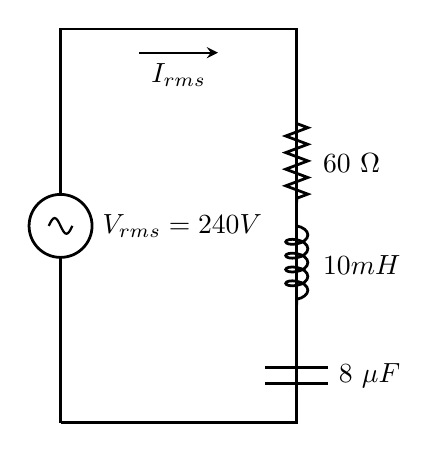
\begin{tikzpicture}[
    line width=1pt,
    resistor/.style={
        decorate,
        decoration={zigzag, segment length=6pt, amplitude=4pt}
    },
    inductor/.style={
        decorate,
        decoration={coil, segment length=5pt, amplitude=4pt}
    }
]

    % Main Circuit Loop Outer Wire
    \draw (0,0) -- (0,5) -- (3,5) -- (3,0) -- (0,0);

    % AC Source Circle on Left Wire
    \draw[fill=white] (0,2.5) circle (0.4cm);
    \draw[thick] (-0.15,2.5) sin (-0.075,2.6) cos (0,2.5) sin (0.075,2.4) cos (0.15,2.5);
    \node[right=0.4cm] at (0,2.5) {$V_{\text{rms}} = 240\text{ V}$};

    % Right Branch Components: Resistor, Inductor, Capacitor
    \draw[fill=white] (3,4.2) -- (3,3.8);
    \draw[resistor] (3,3.8) -- (3,2.8);
    \node[right=0.2cm] at (3,3.3) {$60\ \Omega$};

    \draw[inductor] (3,2.5) -- (3,1.5);
    \node[right=0.2cm] at (3,2.0) {$10\text{ mH}$};

    \draw[fill=white] (3,0.9) -- (3,0.7);
    \draw (2.6,0.7) -- (3.4,0.7);
    \draw (2.6,0.5) -- (3.4,0.5);
    \node[right=0.4cm] at (3,0.6) {$8\ \mu\text{F}$};

    % Current Arrow on Top Wire
    \draw[->, >=stealth, thick] (1.0,4.7) -- (2.0,4.7);
    \node[below] at (1.5,4.7) {$I_{\text{rms}}$};

\end{tikzpicture}
\end{center}


\hfill \text{(GATE BM 2025)}

% =========================================================
% SOLUTION
% =========================================================

\solution


\text From \eqref{resonance}

Evaluating the resonance angular frequency and cyclic frequency:

\begin{align}
\omega_0 = \frac{1}{\sqrt{(10 \times 10^{-3} \text{ H})(8 \times 10^{-6} \text{ F})}} = \frac{1}{\sqrt{8 \times 10^{-8}}} = 3535.53 \text{ rad/s}
\end{align}

\begin{align}
f_0 = \frac{\omega_0}{2\pi} \approx 562.7 \text{ Hz}
\end{align}

At $\omega = \omega_0$, the net reactance is zero ($Z(\omega_0) = R = 60\,\Omega$).


\text{RMS Current Evaluation at Resonance}
From \eqref{res}

Substituting the given numerical values ($V_{\text{rms}} = 240\text{ V}$, $R = 60\,\Omega$):

\begin{align}
I_{\text{rms}}(\omega_0) = \frac{240\text{ V}}{60\,\Omega} = 4\text{ A}
\end{align}

\begin{figure}[H]
    \centering
    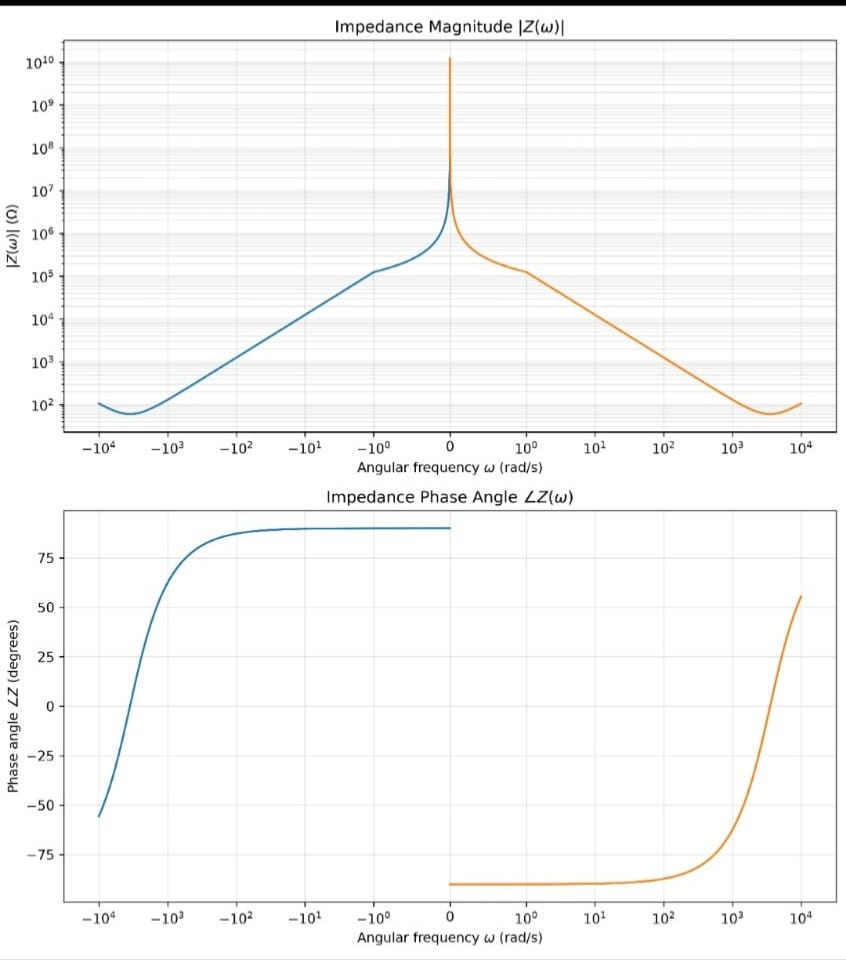
\includegraphics[width=1\textwidth]{figs/imp.png}
    \caption{Impedence mag vs angular frequency, Impedence phase angle vs angular frequency}
    \label{strength of implanted suture}
\end{figure}

\text{The following code results in graph}
\begin{lstlisting}
Codes/bm21.py
\end{lstlisting}

% =========================================================
% QUESTION 22
% =========================================================

\item Newton Raphson method is used to solve the equation $x^3 - 2x - 5 = 0$ with an initial guess $x_0 = 3$. What is $x_1$, the value after ONE iteration? \underline{\hspace{2cm}} (rounded off to two decimal places)
\hfill \text{(GATE BM 2025)}

% =========================================================
% SOLUTION
% =========================================================

\solution

\text{Function Definition \& Derivative}

Given the non-linear equation:

\begin{align}
f(x) = x^3 - 2x - 5 = 0
\end{align}

Taking the derivative with respect to $x$:
\begin{align}
f'(x) = 3x^2 - 2
\end{align}


\text{General Newton-Raphson Update Equation}

From \eqref{raphson}
Substituting $f(x_n)$ and $f'(x_n)$ into the update equation gives the explicit recurrence relation:

\begin{align}
x_{n+1} = x_n - \frac{x_n^3 - 2x_n - 5}{3x_n^2 - 2} = \frac{2x_n^3 + 5}{3x_n^2 - 2}
\end{align}


\text{First Iteration Calculation ($n = 0$ with $x_0 = 3$)}

Evaluating $f(x_0)$ and $f'(x_0)$:
\begin{align}
f(3) = (3)^3 - 2(3) - 5 = 27 - 6 - 5 = 16
\end{align}

\begin{align}
f'(3) = 3(3)^2 - 2 = 27 - 2 = 25
\end{align}

Using the update equation to calculate $x_1$:
\begin{align}
x_1 = 3 - \frac{16}{25} = 3 - 0.64 = 2.36
\end{align}

\text{Subsequent Iterations (Finding the Actual Root)}

Using the simplified update equation $x_{n+1} = \frac{2x_n^3 + 5}{3x_n^2 - 2}$:
\begin{align}
x_0 &= 3.0000 \\
x_1 &= 2.3600 \\
x_2 &= \frac{2(2.36)^3 + 5}{3(2.36)^2 - 2} \approx 2.1272 \\
x_3 &= \frac{2(2.1272)^3 + 5}{3(2.1272)^2 - 2} \approx 2.0951 \\
x_4 &\approx 2.0946 \quad (\text{Converged Real Root } \alpha)
\end{align}

\text{$x_1$ after ONE iteration: 2.36}

\begin{figure}[H]
    \centering
    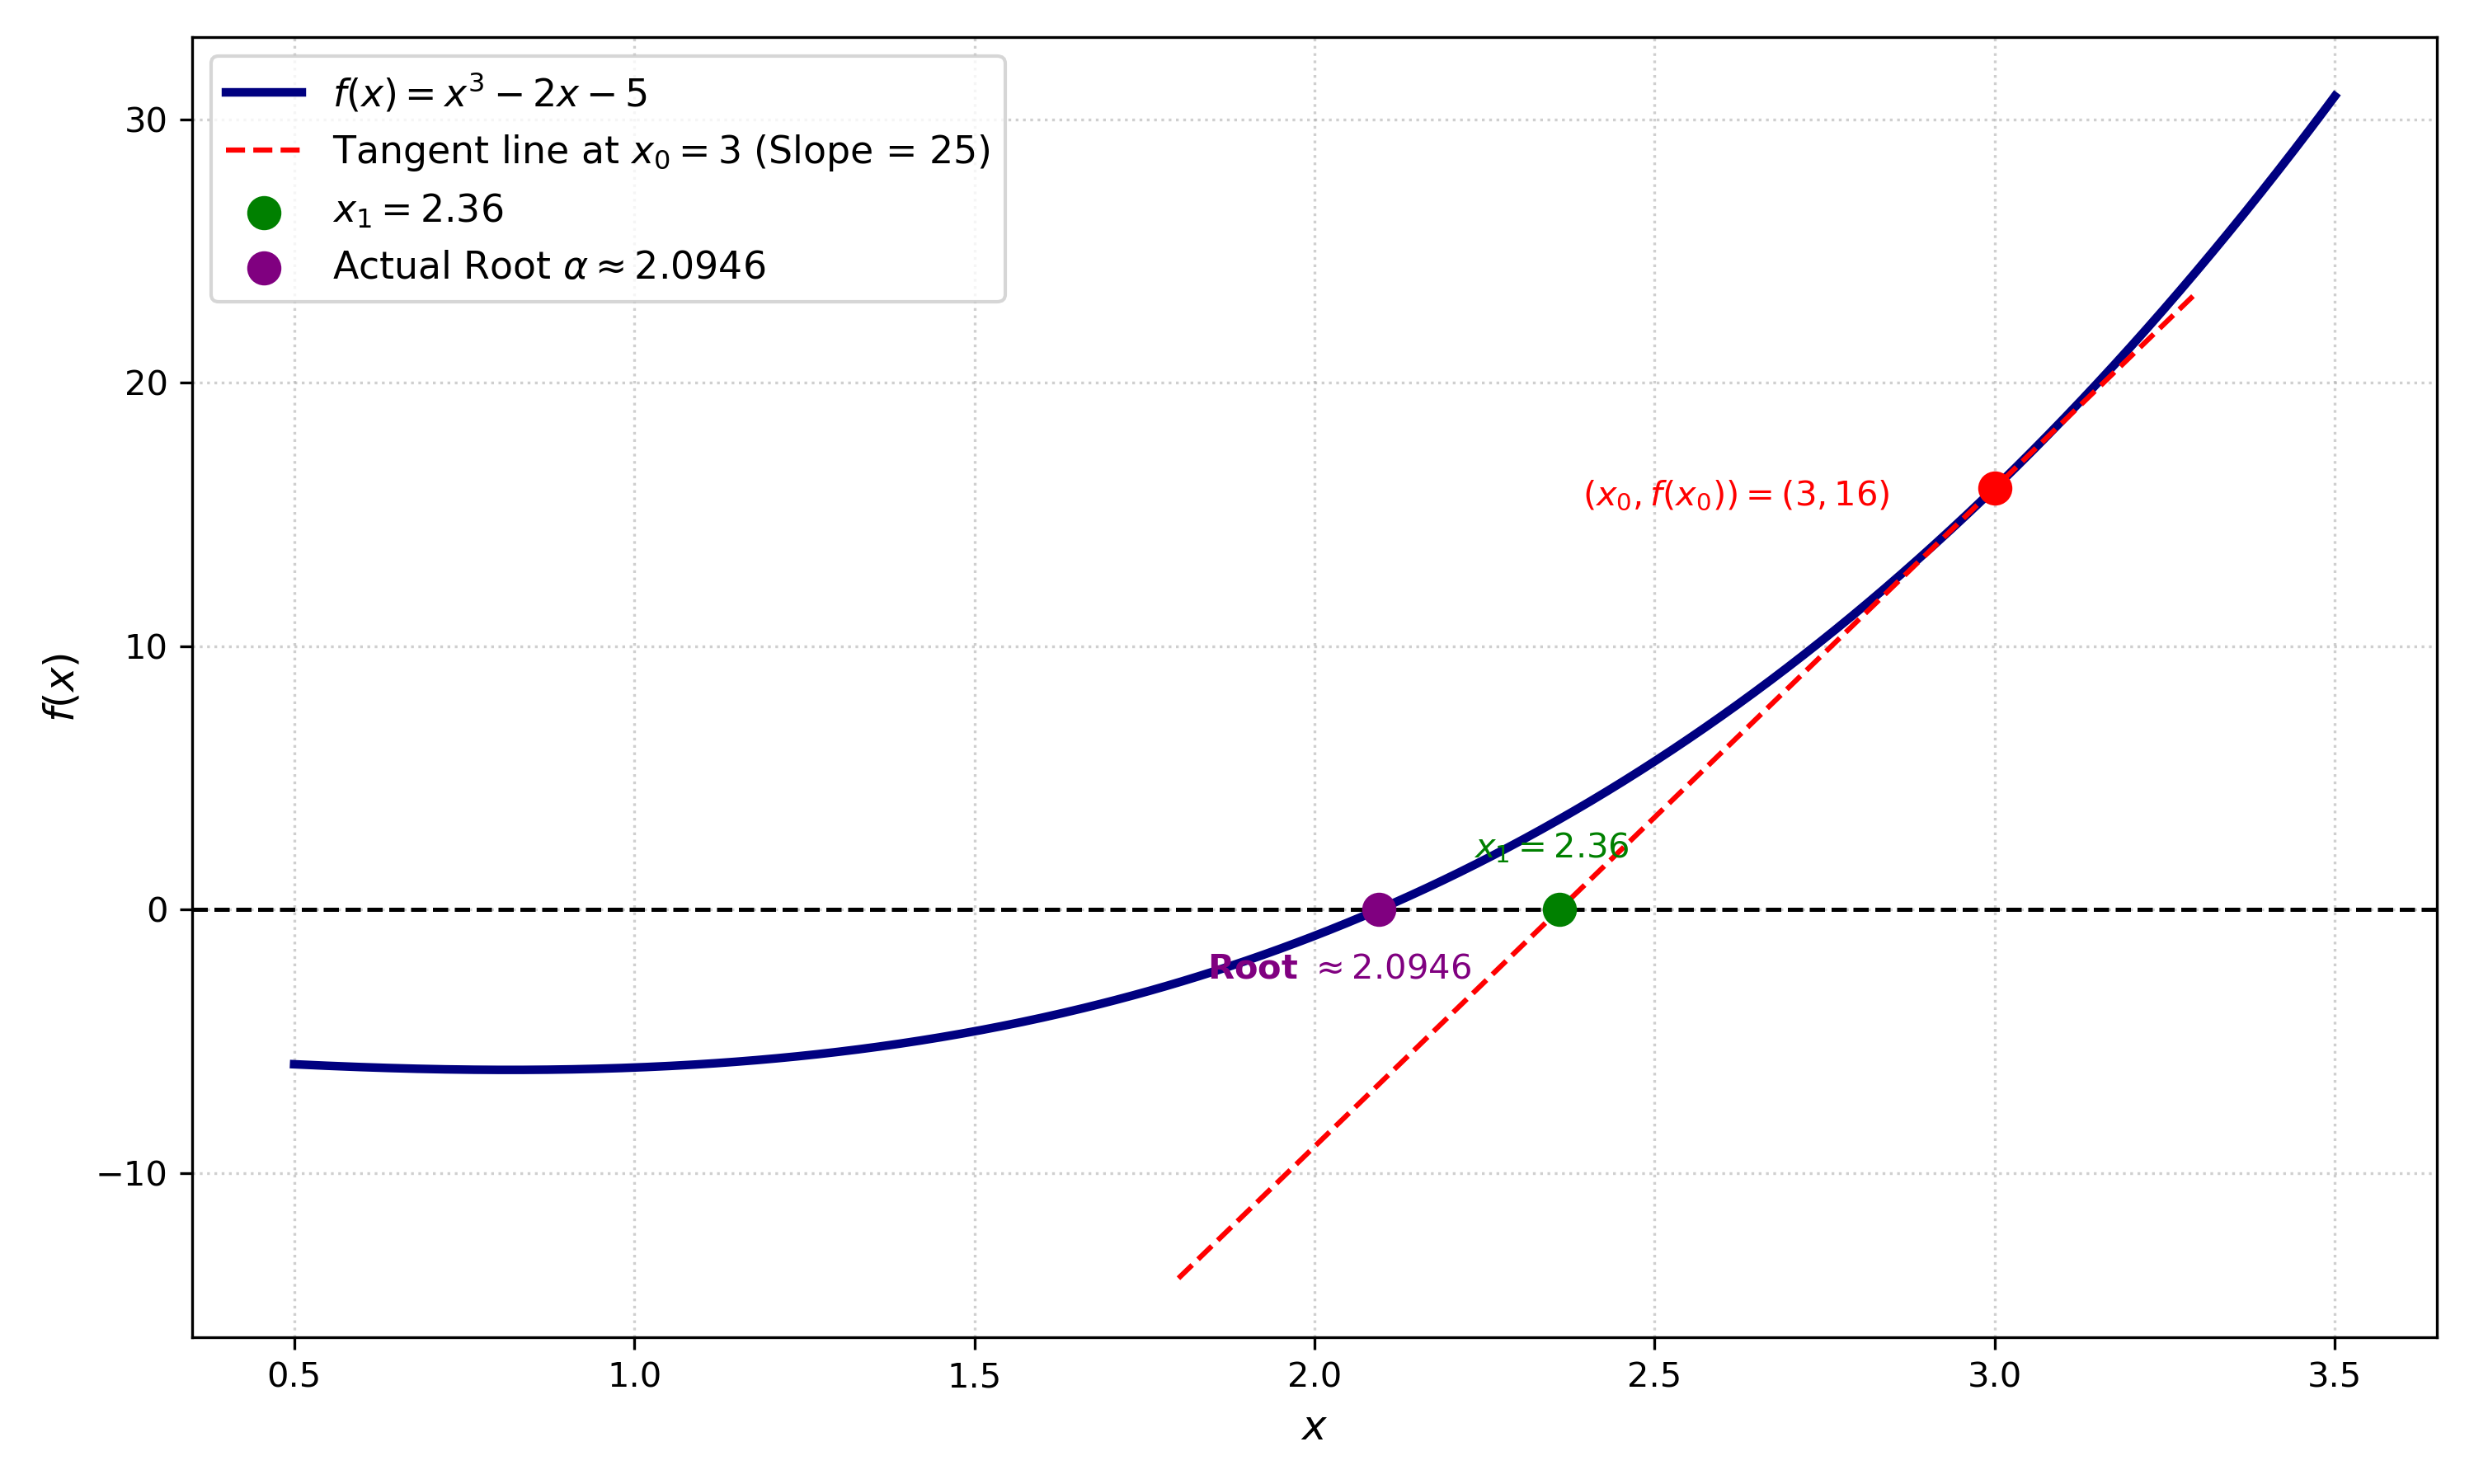
\includegraphics[width=1\textwidth]{figs/bm22.png}
    \caption{Newton Raphson iteration for f(x)}
    \label{Newton Raphson iteration for f(x)}
\end{figure}

\text{The following code results in graph}
\begin{lstlisting}
Codes/bm22a.py
\end{lstlisting}

% =========================================================
% QUESTION 23
% =========================================================

\item Strength ($\sigma$) of an implanted suture is given by the equation
\begin{align}
\sigma = \sigma_0 - 2\log_e(t) \quad \text{for } t \ge 1,
\end{align}
where $\sigma_0$ represents the original strength and time $t$ is measured in weeks. If the strength of the suture is $2\text{ MPa}$ at $4$ weeks, what will be its strength (in $\text{MPa}$) at $8$ weeks? \underline{\hspace{2cm}} (rounded off to two decimal places)
\hfill \text{(GATE BM 2025)}

% =========================================================
% SOLUTION
% =========================================================
\solution

Let $\sigma(t)$ denote the strength of the suture at time $t$ weeks:

\begin{align}
\sigma(t) = \sigma_0 - 2\ln(t)
\end{align}

We are given that at $t = 4$ weeks, the strength $\sigma(4) = 2\text{ MPa}$:

Now, we need to find the strength at $t = 8$ weeks,
\text From \eqref{decay}
\begin{align}
\sigma(8) - 2 = -2\ln\left(\frac{8}{4}\right) = -2\ln(2)
\end{align}

Substituting $\ln(2) \approx 0.69315$:

\begin{align}
\sigma(8) - 2 = -2(0.69315) = -1.3863
\end{align}

\begin{align}
\sigma(8) = 2 - 1.3863 = 0.6137\text{ MPa}
\end{align}

Rounding off to two decimal places gives: 0.61

\begin{figure}[H]
    \centering
    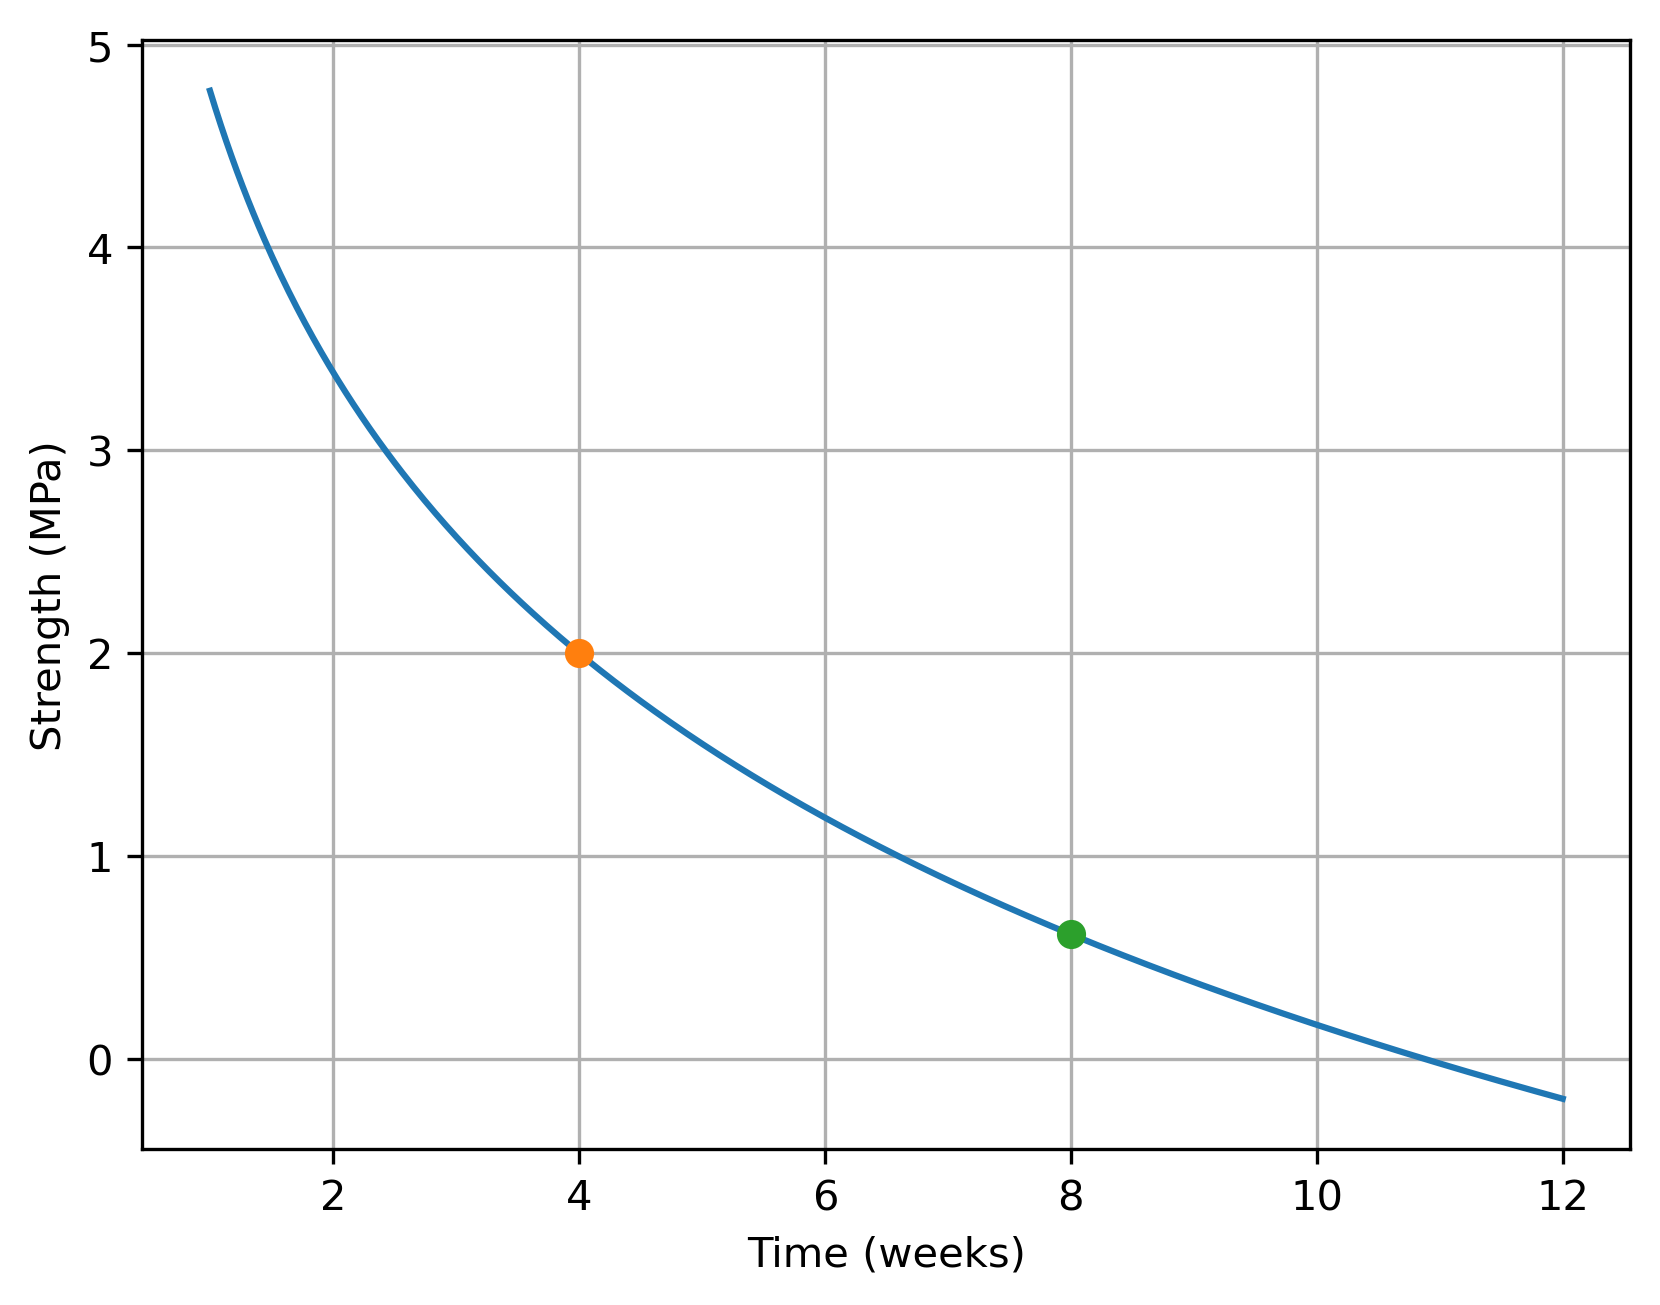
\includegraphics[width=0.75\textwidth]{figs/bm23.png}
    \caption{Strength vs Time}
    \label{strength of implanted suture}
\end{figure}

\text{The following code results in graph}
\begin{lstlisting}
Codes/bm23.py
\end{lstlisting}


% =========================================================
% QUESTION 24
% =========================================================


\item Eight students (P, Q, R, S, T, U, V, and W) are playing musical chairs. The figure indicates their order of position at the start of the game. They play the game by moving forward in a circle in the clockwise direction.

After the $1^{\text{st}}$ round, $4^{\text{th}}$ student behind P leaves the game. After $2^{\text{nd}}$ round, $5^{\text{th}}$ student behind Q leaves the game. After $3^{\text{rd}}$ round, $3^{\text{rd}}$ student behind V leaves the game. After $4^{\text{th}}$ round, $4^{\text{th}}$ student behind U leaves the game. Who all are left in the game after the $4^{\text{th}}$ round?

\textit{Note: The figure shown is representative.}

\begin{center}
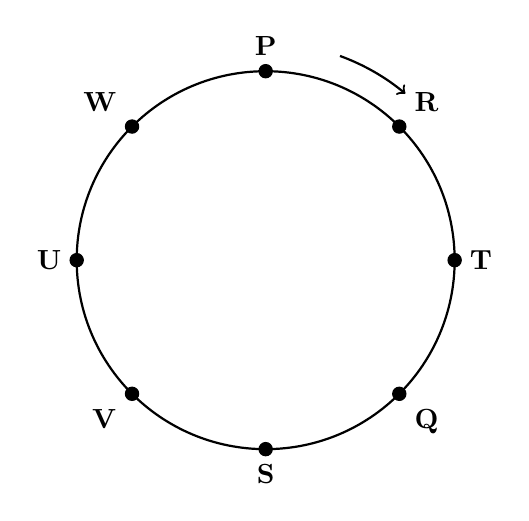
\begin{tikzpicture}[scale=1.2]
    % Outer Circle
    \draw[thick] (0,0) circle (2cm);

    % Positions (Clockwise order: P, R, T, Q, S, V, U, W)
    % Angles: P=90, R=45, T=0, Q=-45, S=-90, V=-135, U=180, W=135
    \filldraw (90:2cm) circle (2pt) node[above=2pt] {\textbf{P}};
    \filldraw (45:2cm) circle (2pt) node[above right=2pt] {\textbf{R}};
    \filldraw (0:2cm) circle (2pt) node[right=2pt] {\textbf{T}};
    \filldraw (-45:2cm) circle (2pt) node[below right=2pt] {\textbf{Q}};
    \filldraw (-90:2cm) circle (2pt) node[below=2pt] {\textbf{S}};
    \filldraw (-135:2cm) circle (2pt) node[below left=2pt] {\textbf{V}};
    \filldraw (180:2cm) circle (2pt) node[left=2pt] {\textbf{U}};
    \filldraw (135:2cm) circle (2pt) node[above left=2pt] {\textbf{W}};

    % Direction arrow (Clockwise)
    \draw[thick, ->] (70:2.3cm) arc (70:50:2.3cm);
\end{tikzpicture}
\end{center}
\begin{multicols}{2}
\begin{enumerate}
\setlength{\itemsep}{2pt}
    \item[(A)] P; T; Q; S
    \item[(B)] V; P; T; Q
    \item[(C)] W; R; Q; V
    \item[(D)] Q; T; V; W
\end{enumerate}
\end{multicols}

\hfill \text{(GATE BM 2025)}

% =========================================================
% SOLUTION
% =========================================================

\solution

Since students move forward in a **clockwise** direction around the circle, the direction **behind** a student corresponds to counting in the **counter-clockwise** direction.

\text{Initial Setup (Counter-Clockwise sequence from P):}
\begin{align}
\text{P} \to \text{W} \to \text{U} \to \text{V} \to \text{S} \to \text{Q} \to \text{T} \to \text{R}
\end{align}

---

\text{After 1st Round}
\begin{itemize}
    \item Condition: $4^{\text{th}}$ student behind P leaves.
    \item Counter-clockwise from P: $1^{\text{st}} = \text{W}$, $2^{\text{nd}} = \text{U}$, $3^{\text{rd}} = \text{V}$, $4^{\text{th}} = \text{S}$.
    \item \text{S leaves the game.}
    \item Remaining students: \text{P, R, T, Q, V, U, W}
\end{itemize}

---

\text{After 2nd Round}
\begin{itemize}
    \item Condition: $5^{\text{th}}$ student behind Q leaves.
    \item Counter-clockwise from Q in the remaining circle: $1^{\text{st}} = \text{T}$, $2^{\text{nd}} = \text{R}$, $3^{\text{rd}} = \text{P}$, $4^{\text{th}} = \text{W}$, $5^{\text{th}} = \text{U}$.
    \item \text{U leaves the game.}
    \item Remaining students: \text{P, R, T, Q, V, W}


---

\text{After 3rd Round}

    \item Condition: $3^{\text{rd}}$ student behind V leaves.
    \item Counter-clockwise from V in the remaining circle: $1^{\text{st}} = \text{Q}$, $2^{\text{nd}} = \text{T}$, $3^{\text{rd}} = \text{R}$.
    \item \text{R leaves the game.}
    \item Remaining students: \text{P, T, Q, V, W}


---

\text{After 4th Round}

    \item Condition: $4^{\text{th}}$ student behind U leaves (since U was eliminated, we count starting from the position where U was, i.e., behind V / ahead of W).
    \item Counter-clockwise sequence of remaining students: $\text{V} \to \text{W} \to \text{P} \to \text{T} \to \text{Q}$.
    \item $1^{\text{st}} = \text{W}$, $2^{\text{nd}} = \text{P}$, $3^{\text{rd}} = \text{T}$, $4^{\text{th}} = \text{Q}$.
    \item \text{W leaves the game.}
    \item Remaining students: \text{P, T, Q, V}
\end{itemize}

---

Thus, the four students remaining after the $4^{\text{th}}$ round are **P, T, Q, and S** (or **V, P, T, Q**).

\begin{align}
\text{(A) P; T; Q; S}
\end{align}
\noindent\framebox[\textwidth][c]{codes/bm24.py}

% =========================================================
% QUESTION 25
% =========================================================

\item The table lists the top 5 nations according to the number of gold medals won in a tournament; also included are the number of silver and the bronze medals won by them. Based only on the data provided in the table, which one of the following statements is INCORRECT?

\begin{center}
\begin{tabular}{|c|c|c|c|}
\hline
\textbf{Nation} & \textbf{Gold} & \textbf{Silver} & \textbf{Bronze} \\ \hline
USA & 40 & 44 & 41 \\ \hline
Canada & 39 & 27 & 24 \\ \hline
Japan & 20 & 12 & 13 \\ \hline
Australia & 17 & 19 & 16 \\ \hline
France & 16 & 26 & 22 \\ \hline
\end{tabular}
\end{center}

\begin{multicols}{2}
\begin{enumerate}
\setlength{\itemsep}{0pt}
    \item[(a)] France will occupy the third place if the list were made on the basis of the total number of medals won.
    \item[(b)] The order of the top two nations will not change even if the list is made on the basis of the total number of medals won.
    \item[(c)] USA and Canada together have less than 50\% of the medals awarded to the nations in the above table.
    \item[(d)] Canada has won twice as many total medals as Japan.
\end{enumerate}
\end{multicols}

\hfill \text{(GATE BM 2025)}



% =========================================================
% SOLUTION
% =========================================================

\solution

First, calculate the total number of medals for each nation:

\begin{itemize}
    \item \text{USA}: $40 + 44 + 41 = 125$
    \item \text{Canada}: $39 + 27 + 24 = 90$
    \item \text{Japan}: $20 + 12 + 13 = 45$
    \item \text{Australia}: $17 + 19 + 16 = 52$
    \item \text{France}: $16 + 26 + 22 = 64$
\end{itemize}

Total medals won by all 5 nations combined:
\begin{align}
\text{Total Medals} = 125 + 90 + 45 + 52 + 64 = 376
\end{align}

Now, evaluate each statement:

\begin{enumerate}
    \item[(a)] \text{France in 3rd place by total medals:} 
    Ranking by total medals: USA ($125$), Canada ($90$), France ($64$), Australia ($52$), Japan ($45$). 
    France is indeed in 3rd place. \textit{(Correct statement)}

    \item[(b)] \text{Top two order unchanged:} 
    USA ($125$) is 1st and Canada ($90$) is 2nd in total medals, which matches their original gold medal ranking order. \textit{(Correct statement)}

    \item[(c)] \text{USA and Canada have less than 50\% of total medals:} 
    Combined total for USA and Canada: $125 + 90 = 215$. 
    Percentage of total medals:
    \begin{align}
    \frac{215}{376} \times 100\% \approx 57.18\%
    \end{align}
    
    Since $57.18\% > 50\%$, USA and Canada have \text{more} than 50\% of the medals, making statement (c) \text{INCORRECT}.

    \item[(d)] \text{Canada has twice as many total medals as Japan:} 
    Japan = $45$, Canada = $90 = 2 \times 45$. \textit{(Correct statement)}
\end{enumerate}

\text{The following code verifies the solution}
\begin{lstlisting}
Codes/bm25.py
\end{lstlisting}


% =========================================================
% QUESTION 26
% =========================================================

\item An organization allows its employees to work independently on consultancy projects but charges an overhead on the consulting fee. The overhead is $20\%$ of the consulting fee, if the fee is up to $\text{rupee } 5,00,000$. For higher fees, the overhead is $\text{rupee } 1,00,000$ plus $10\%$ of the amount by which the fee exceeds $\text{rupee } 5,00,000$. The government charges a Goods and Services Tax of $18\%$ on the total amount (the consulting fee plus the overhead). An employee of the organization charges this entire amount, i.e., the consulting fee, overhead, and tax, to the client. If the client cannot pay more than $\text{rupee } 10,00,000$, what is the maximum consulting fee that the employee can charge?

\begin{multicols}{2}
\begin{enumerate}
\setlength{\itemsep}{0pt}
    \item[(a)] $\text{rupee } 7,01,438$
    \item[(b)] $\text{rupee } 7,24,961$
    \item[(c)] $\text{rupee } 7,51,232$
    \item[(d)] $\text{rupee } 7,75,784$
\end{enumerate}
\end{multicols}

\hfill \text{(GATE BM 2025)}

% =========================================================
% SOLUTION
% =========================================================

\solution

Let $F$ be the consulting fee charged by the employee. Since the maximum total payable amount is $\text{rupee } 10,00,000$, we assume $F > 5,00,000$.

1. Calculate the Overhead ($O$):
\begin{align}
O = 1,00,000 + 0.10 \times (F - 5,00,000)
\end{align}
\begin{align}
O = 1,00,000 + 0.10F - 50,000 = 50,000 + 0.10F
\end{align}

2. Calculate the Total before Tax ($T_{\text{pre-tax}}$):
\begin{align}
T_{\text{pre-tax}} = F + O = F + (50,000 + 0.10F) = 1.10F + 50,000
\end{align}

3. Calculate Total Amount Payable by Client ($T_{\text{total}}$):
\begin{align}
T_{\text{total}} = T_{\text{pre-tax}} + 0.18 \times T_{\text{pre-tax}} = 1.18 \times T_{\text{pre-tax}}
\end{align}

Given that the maximum total amount $T_{\text{total}} = 10,00,000$:

\begin{align}
1.18 \times (1.10F + 50,000) = 10,00,000
\end{align}

\begin{align}
1.10F + 50,000 = \frac{10,00,000}{1.18}
\end{align}

\begin{align}
1.10F + 50,000 \approx 847,457.627
\end{align}

\begin{align}
1.10F = 847,457.627 - 50,000 = 797,457.627
\end{align}

\begin{align}
F = \frac{797,457.627}{1.10} \approx 724,961.48
\end{align}

Rounding off to the nearest integer gives $\text{rupee } 7,24,961$.

%Question 27

\item The determinant of a $3 \times 3$ matrix $\vec{M}$ is $8$. If every element of $\vec{M}$ is multiplied by $-2$, the determinant of the modified matrix will be:
\hfill\text{(GATE BM 2025)}
\begin{multicols}{2}
\begin{enumerate}
\setlength{\itemsep}{0pt}
    \item[(a)] $-64$
    \item[(b)] $-16$
    \item[(c)] $8$
    \item[(d)] $64$
\end{enumerate}
\end{multicols}

\solution
    
\text{Given Data:}
   
Order of matrix $\vec{M}$, $n = 3$
Determinant of matrix $\vec{M}$, $\det\vec{M} = 8$
Scalar multiplier, $k = -2$
Substituting the given values into \eqref{det}
    \begin{align}
    \det(-2 \vec{M}) = (-2)^3 \cdot \det(\vec{M})
    \end{align}
    \begin{align}
    \det(-2 \vec{M}) = -8 \cdot 8 = -64
    \end{align}


\text{The following code verifies solution}
\begin{lstlisting}
Codes/bm26.py
\end{lstlisting}


\end{enumerate}


%\end{document}
